\documentclass[11pt,a4paper]{paper} %taille WP BCE
\usepackage[T1]{fontenc}
%\usepackage[latin1]{inputenc}
%\usepackage{amssymb,amsmath,a4wide}
\usepackage[utf8]{inputenc}
\usepackage{amssymb,amsmath}
\usepackage{nicefrac}
\usepackage[pdftex]{graphicx}
\usepackage{ctable}
\usepackage{amsmath}
%\usepackage{threeparttable} %na
%\usepackage{tabu} %na
\usepackage{tabularx}
\usepackage{subfig}
\usepackage{rotating}
\usepackage{longtable}
%\usepackage[table]{xcolor} % clash with floatrow
\usepackage{xcolor} 
\usepackage{floatrow}
\usepackage{threeparttable}
%\usepackage[multiple]{footmisc} %na
\usepackage{bm}
\usepackage{fancybox}
%\usepackage{harvard}
\usepackage{geometry}         % Definir les marges
\geometry{verbose,a4paper,tmargin=3.5cm,bmargin=3.5cm,lmargin=2.5cm,rmargin=2.5cm}
\usepackage{setspace}
%\usepackage{ccaption}
\usepackage[colorlinks=true,citecolor=black, urlcolor=black, linkcolor=black]{hyperref}
\usepackage{url}
\newcommand{\email}[1]{\href{mailto:#1}{\nolinkurl{#1}}}
\usepackage[french, english]{babel}  % Placez ici une liste de langues, la derniere etant la langue principale
\usepackage{lscape}
\usepackage{afterpage}
\usepackage{supertabular}    %na            %  mettre pour les grands tableaux en formant paysage. marche avec \begin{landscape}
% style de la biblio : necessaire pour utiliser BibTex, necessite le deuxieme fichier exemple.bib
\usepackage{caption}
%\usepackage[longnamesfirst]{natbib}
\usepackage[round,sort]{natbib}
\newcommand{\tqdl}{\textquotedblleft}
\newcommand{\tqdr}{\textquotedblright}
\DeclareUnicodeCharacter{FB01}{fi}
\DeclareUnicodeCharacter{FB00}{ff}
%\linespread{1.2}
\usepackage{setspace}
\setstretch{1.5} % BCE line spacing 1.5
%\doublespacing
\pagenumbering{gobble} %BCE: NO PAGE NUMBERS, nor any other items in the page headers or footers
%\usepackage[hmargin=2.5cm,vmargin=3.5cm]{geometry} %BCE: The margins are 2.5 cm (horizontal) and 3.5 cm (vertical)


% !TeX spellcheck = en_US


\begin{document}
\title{Estimating the elasticity of consumer prices to the exchange rate: an accounting approach	\thanks{We thank Marion Cochard, Pavel Diev, Hubert Escaith, Guillaume Gaulier, Yannick Kalantzis, Guy Levy-Rueff, Sébastien Miroudot, Jean-François Ouvrard, François de Soyres and an anonymous referee for comments and suggestions, as well as participants at Banque de France seminars. Any remaining errors are ours. All programs are available at \url{https://github.com/gdaudin/OFCE_CommerceVA}. Data and results are available upon request.}\\
\vspace{1cm}
}
\vspace{1cm}
\date{\today}
\author{
	Hadrien Camatte\thanks{Banque de France. E-mail: \email{hadrien.camatte@banque-france.fr}}
	\and
	Guillaume Daudin\thanks{Université Paris-Dauphine, PSL University, CNRS, 8007, IRD, 260, LEDa, DIAL, 75016, Paris, France. Sciences Po, OFCE, 75007, Paris. Corresponding author. E-mail: \email{guillaume.daudin@dauphine.psl.eu}}
	\and
	Violaine Faubert\thanks{Banque de France, ECB. E-mail: \email{violaine.faubert@ecb.europa.eu}}
	\and
	Antoine Lalliard\thanks{Banque de France. E-mail: \email{antoine.lalliard@banque-france.fr}}
	\and
	Christine Rifflart\thanks{Sciences Po, OFCE. E-mail: \email{christine.rifflart@sciencespo.fr}}
}
\maketitle

%\vspace*{\fill}
\newpage % BCE: abstract sur une nouvelle page

\begin{abstract}
{\small \noindent
%We focus on cost-push inflation through global value chains.
%We build on three sectoral world input-output datasets (WIOD and two versions of TiVA). We assume a Cobb-Douglas production framework and work in a partial equilibrium setting.
We analyse the elasticity of the household consumption expenditure (HCE) deflator to the exchange rate, using world input-output tables (WIOT) from 1995 to 2019. 
In line with the existing literature, we find a modest output-weighted elasticity of around 0.1.
This elasticity is stable over time but heterogeneous across countries, ranging from 0.05 to 0.22. 
Such heterogeneity mainly reflects differences in foreign product content of consumption and intermediate products. 
Direct effects through imported consumption and intermediate products entering domestic production explain most of the transmission of an exchange rate appreciation to domestic prices.
By contrast, indirect effects linked to participation in global value chains play a limited role. 
Our results are robust to using four different WIOT datasets. 
As WIOT are data-demanding and available with a lag of several years, we extrapolate a reliable estimate of the HCE deflator elasticity from 2015 onwards using trade data and GDP statistics. 
%VF a GD: je propose un abstract plus general car on a pas encore introduit les diferences entre bases de donnes et le lecteur risque de ne pas comprendre les references a WIOD et MRIO dans l'abstract. Je suggere d'etre plus detaille dans l'introductio
%This yields an estimate of the elasticity very close to the one computed from MRIO WIOT.

% Abstract WP BdF
%We contribute to the debate on the global determinants of domestic prices by investigating cost-push inflation through global value chains. We confirm the importance of global value chains in channelling external shocks to consumer price inflation. Using data from WIOD on a sample of 43 countries, we find that the mean output-weighted elasticity of consumer prices increased in absolute value from 0.075 in 2000 to 0.094 in 2008. After peaking in 2008, it declined to 0.088 in 2014. Extrapolations suggest that this continued until 2016, before reversing in 2017 and 2018. Our findings are robust to using three different datasets.	
		
%%Original abstract: decomment once	
%Following the 2008 financial crisis, inflation rates in advanced economies have been at odds with the prediction of a standard Phillips curve. 
%This puzzle has triggered a debate on the global determinants of domestic prices.
%We contribute to this debate by investigating the impact of exchange rate shocks on consumer prices from 1995 to 201. 
%We focus on cost-push inflation through global value chains.
%We build on three sectoral world input-output datasets (WIOD and two versions of TiVA). We assume a Cobb-Douglas production framework and work in a partial equilibrium setting.
%The construction of World Input-Output tables is data-demanding and WIOTs are typically released with a lag of several years. 
%To address this gap, we use more up-to-date GDP and trade data, thus providing a tool for approximating the partial equilibrium impact of an exchange rate shock on consumer prices from 2015 onwards.
%Depending on countries, the absolute value of the elasticity of the household consumption expenditure (HCE) deflator to the exchange rate ranges from 0.05 to 0.35, confirming the importance of global value chains in channelling external shocks to domestic inflation.
%%Most of the propagation of shocks passes through imported consumer goods and domestic input-output linkages.
%Using data from WIOD on a sample of 43 countries, we find that the mean output-weighted elasticity of the HCE deflator to the exchange rate increased in absolute value from 0.075 in 2000 to 0.094 in 2008. 
%After peaking in 2008, it declined to 0.088 in 2014.
%Extrapolations based on more up-to-date GDP and trade data suggest that the decline continued until 2016, before reversing in 2017 and 2018. 
%Our findings are robust to using three different datasets.
%%Both recent versions of TIVA yield a similar evolution.
%%Our approach suffers from a limitation: world input-output databases are only available after a sizeable time delay.
%%The latest data date back to 2015. 
%%To address this, we use up-to-date GDP and trade data to extrapolate the impact of exchange rate shock on consumer prices.
%%Finally, we establish that the results obtained using sectoral world input-output datasets up to 2015 can be extrapolated to recent years thanks to the use of easily obtainable statistics as GDP and trade statistics. 

%%Firms' participation in global value chains strengthens cross-country linkages via trade in intermediate inputs. 
%%In this paper, we build on three sectoral world input-output datasets  to assess the role of global input-output linkages in the propagation of exchange rate shocks in the international economy. 
%% %à faire: productivity shocks More specifically, we study the role of global input-output linkages in transmitting oil prices shocks across economies.
%%We examine the increasing integration of the European economies since the adoption of the common currency and investigate whether the shortening of global value chains in the wake of the Great Recession has changed the propagation of global price shocks. We provide evidence that, following an appreciation of the domestic currency, the direct effect of global price shocks, i.e. the effect resulting from the share of imported final and intermediate goods in domestic consumption, explains the bulk of the propagation of global shocks to domestic consumer prices. By contrast, we find a limited role for the additional transmission of lower domestic input prices to other sectors of the domestic economy and other countries occurring during subsequent production cycles. Finally, building on sectoral data, we examine which sectors experience higher spillovers from global price shocks.
%%%We also contribute to the literature on global input-output linkages by assessing whether results are consistent across the different world input output databases available (WIOD and TiVA).
}

{\small \bigskip \noindent \emph{JEL Classification}\/: C67, E31, F42, F62\\}
{\small \noindent \emph{Keywords}\/: input-output linkages, spillovers, global value chains, cost-push inflation \\ }
\end{abstract}


%Ajout non technical summary sur nouvelle page
\newpage
\begin{center}
  {\bfseries Non-technical summary}
\end{center}
\bigskip
%importance de la question pour le public et la politiaue monetaire
%A country’s import, producer or consumer prices change in response to a variation in its exchange rate. 
Understanding the influence of exchange rate on inflation is critically important for setting monetary policy and measuring the extent of expenditure switching that follows exchange rate variations, which, in turn, has an impact on real activity.\\
%Data
In this paper, we analyse the impact of exchange rate variations on domestic consumer prices using several datasets covering most advanced and emerging economies, from 1995 to 2019. 
%Method
We perform an accounting exercise based on information contained in world input-output tables, by way of large matrices inversions.
Our accounting approach helps identifying which countries and sectors are under pressure to adjust their prices when subject to an exchange rate variation.\\
%We assume a Cobb-Douglas production framework where firms have a simple cost-minimising behaviour and work in a partial equilibrium setting.
%First, we assume that exchange rate fluctuations completely pass-through to import prices. 
%Hence, wo do not consider the fact that the pass-through might be incomplete, as suggested by a large body of literature (see for example \cite{Berman2012}).
%Using alternative exchange rate pass-through assumptions would thus entail lower elasticity values. 
%Second, we assume that all pricings occur using the currency of the producing country (in line with the ‘producer currency pricing’ paradigm). 
%However, a large body of empirical literature suggests that the vast majority of trade is invoiced in a small number of ‘dominant currencies,’ with the U.S. dollar playing a major role. The ‘dominant currency paradigm’ (\cite{Gopinath2020}) implies that for non-U.S. countries, the exchange rate pass-through into import prices (in home currency) should be high and driven by the dollar exchange rate as opposed to the bilateral exchange rate, whereas for the U.S. the pass-through into import prices should be low.
%We also assume that the exchange rate shock is proportional across sectors. 
%Variation élasticite dans le temps et l'espace
Our main findings are fourfold. 
First, we document the evolution over time of the impact of exchange rate variations on consumer prices.
In line with the existing literature, we find that in response to a 1\% appreciation of the domestic currency, domestic consumer prices decrease by arround 0.10\% on average at the world level. 
The impact of exchange rate variations on consumer prices has remained broadly stable over the past two decades.
This modest estimate is likely an upper bound. Indeed, we make two assumptions to simplify our computations. \\
We assume that exchange rate fluctuations completely pass-through to import prices.
However, a large body of literature suggests that the pass-through is incomplete, even in the long run, as a result of slow nominal price adjustments or the pricing-to-market behaviour of firms (see \cite{Ozyurt2016} for a discussion of the literature).
For example, the pass-through depends on the intensity of competition in domestic markets: while an exchange rate appreciation lowers the price of imported inputs, a firm with limited competitive pressure may avail of greater profit margins rather than reduce prices in an effort to maintain its market share.
Hence, pricing-to-market strategies of exporters aiming to defend their market shares would imply a lower exchange rate pass-through. \\
In addition, we work under the producer pricing assumption.
However, in large and attractive markets, competitive pressures may push producers to adopt local currency pricing strategies, where exporting firms adapt their mark-ups depending on the destination market to offset exchange rate movements. 
Under the local currency pricing paradigm, prices are thus sticky in the currency of the destination market.
%Settlement and invoicing of imports in the domestic currency is another factor weakening the elasticity of domestic prices to the exchange rate.
Hence, using alternative pricing assumptions would entail lower estimates of the percentage change in consumer prices in response to a 1\% change in the exchange rate. \\
%Using the WIOD database, which covers a sample of 43 countries, we find that the mean GDP-weighted elasticity of consumer prices to the exchange rate increased from 0.08 in 2000 to 0.09 in 2008. 
%After peaking in 2008, the elasticity slightly declined between 2009 and 2015. \\
%Using the MRIO database, which provides data up to 2018, we find that the elasticity has bounced back from 2015 onwards. However, the MRIO database suffers from data quality issues in 2018 and is likely unreliable for this year (see online Appendix F).\\
%Our finding concurs with the literature. Using comprehensive measures of global value chain integration, \cite{Timmer2016} find that the expansion of global value chain has slowed since the 2008-2009 Great Recession.
The impact of a 1\% exchange rate fluctuation on domestic prices is heterogeneous across countries. 
It ranges from 0.05\% to 0.22\%, reflecting different degrees of openness to trade. 
In the euro area, the impact is close to 0.10 in Italy, France, Germany, Spain, Portugal and Greece, whereas it is twice higher for small open economies like Luxembourg, Malta, Slovakia and Ireland.
We also estimate the impact of an appreciation of the US dollar on its trading partners.
The highest impacts are observed for the US's major trading partners (Canada, Mexico and Ireland).\\
% Impact par secteur
Second, we examine which sectors experience higher spillovers from an exchange rate appreciation. 
Non-energy industrial goods explain the bulk of the impact of an exchange rate variation on consumer prices. 
Services also play a significant role, especially in advanced economies such as the US, Japan, Germany and France. 
Although services are mainly produced domestically and do not rely much on imported inputs, they account for a substantial share of total consumption.
Thus, even small price changes have a large effect on the HCE deflator.\\
%Decomposition et canaux de transmission
Third, we analyse the role of global value chains in the transmission of an exchange rate appreciation to consumer prices. 
When production processes are global, an exchange rate appreciation impacts consumer prices through four distinct channels: \textit{i)} the prices of imported final goods sold directly to domestic consumers;
\textit{ii)} the prices of imported inputs entering domestic production; 
%Hence, a currency appreciation reduces the price of imported inputs, and thus further reduces domestic consumer prices. 
\textit{iii)} the price of exported inputs feeding through imported foreign production;
\textit{iv)}, changes in domestic and foreign production costs in turn passing through to the price of inputs for domestic and foreign goods and causing further production costs variations through input-output linkages.\\
We find that the first two channels explain three quarters of the transmission of an exchange rate appreciation to domestic prices.
The last two channels, which reflect the impact of participation in global value chains, play a limited role, with marked across-countries heterogeneity.\\
%Extrapolation
Fourth, we show that a precise assessment of the impact of exchange rate variations on consumer prices can be estimated without resorting to world input output tables. 
The construction of World Input-Output tables is data-demanding and WIOTs are typically released with a lag of several years. 
As a result, most WIOTs are not available for the most recent years.
% meme commentaire: on n'a pas introduit les differentes bases de donnees
To fill the data gap, we extrapolate the impact of exchange rate variations on consumer prices using up-to-date GDP and trade statistics.
We obtain a reliable estimate.
We thus provide a simple accounting tool to estimate the percentage change in prices in response to exchange rate variations for the most recent years. We hope this will help explain and improve the variety of inflation elasticities to the exchange rate used in forcasting models.\\

\newpage 
\section*{Introduction}
%Nouvelle intro avril 2021 ou non technical summary
This paper studies on the elasticity of the household consumption expenditure (HCE hereafter) deflator to the exchange rate. 
%Data
We analyse the composition and determinants of the HCE deflator elasticity using world input-output tables (WIOT hereafter) covering twenty years of data, from 1995 to 2019.
For the sake of robustness, we use several datasets (WIOD, two distinct releases of the OECD TiVA database and the MRIO database developed by the Asian Development Bank). 
%Method
We perform an accounting exercise based on information contained in WIOTs with large matrices inversion. 
%We assume a Cobb-Douglas production framework where firms have a simple cost-minimising behaviour and work in a partial equilibrium setting.
We make two assumptions to simplify our computations. 
First, we assume a full exchange rate pass-through to import prices. 
Hence, we do not consider the fact that the pass-through might be incomplete, as suggested by a large body of literature (see for example \cite{Berman2012}).
%Hence, we do not consider other relevant determinants of the exchange rate pass-through.
%For instance, pricing-to-market strategies of exporters aiming to defend their market shares would imply a lower exchange rate pass-through.
%Similarly, settlement and invoicing of imports in the domestic currency is another factor likely to weaken the elasticity of domestic prices to exchange rate movements.
As a result, our estimates provide an upper bound of the HCE deflator elasticity.
Using alternative pricing assumptions would entail lower values.
%For instance, assuming that only 60\% of invoices in the euro area goods trade are denominated in foreign currency (see \cite{Ortega2020}) would entail lower elasticity values. 
Second, we suppose that all pricings occur using the currency of the producing country, despite the well-documented role of dominant-currency pricing (\cite{Gopinath2020}).
As a consequence of these two assumptions, we also assume that the impact of the exchange rate fluctuation is proportional across sectors.
Despite these simplifying assumptions, our estimates provide an accounting-based gauge of how large the elasticity of consumer prices to the exchange rate could be, considering direct and indirect import content in consumption and global value chain linkages. 
This accounting approach helps identifying which countries and sectors are under pressure to adjust their prices when subject to an exchange rate variation.  \\
%Variation élasticite dans le temps et l'espace
Our contribution to the literature is fourfold. 
First, we analyse the evolution of the elasticity of the HCE deflator to the exchange rate. We document differences across countries.
We pay particular attention to the heteregeneity observed in the euro area, reflecting different degrees of openness to trade. \\
% Impact par secteur
Second, building on sectoral data, we examine which sectors experience higher spillovers from an appreciation of the national currency. 
We focus on the main components of the HCE deflator, i.e. manufacturing goods, services, food and energy. 
We analyse the contribution of these different products to the HCE deflator elasticity and document cross-country heterogeneity in the elasticity.\\
%Decomposition et canaux de transmission
Third, we look into the determinants of the HCE deflator elasticity and the role of global value chains in the transmission of an exchange rate appreciation. 
We identify four channels through which the exchange rate impacts the HCE deflator when production processes are global: \textit{i)} the prices of imported final goods sold directly to domestic consumers;
\textit{ii)} the prices of imported inputs entering domestic production; 
%Hence, a currency appreciation reduces the price of imported inputs, and thus further reduces domestic consumer prices. 
\textit{iii)} the price of exported inputs feeding through imported foreign production;
\textit{iv)} changes in domestic and foreign production costs in turn passing through to the price of inputs for domestic and foreign goods, causing further changes in production costs through input-output linkages.
We find that the first two channels explain three-quarters of the transmission of an exchange rate appreciation to domestic prices.
By contrast, the last two channels, which reflect the impact of global value chains, play a more limited role, with marked cross-countries heterogeneity.
Hence, only one-fourth of the elasticity of the HCE deflator to the exchange rate is attributable to participation in global value chains.\\
%Extrapolation
Fourth, we show that a precise assessment of the HCE deflator elasticity to the exchange rate can be estimated for recent years without resorting to WIOTs. 
The construction of World Input-Output tables is data-demanding and WIOTs are typically released with a lag of several years.
As a result, WIOT are not available for the most recent years. For instance, the latest WIOD dataset dates back to 2014. 
Although the MRIO dataset covers most recent years, it suffers from data quality issues in 2018. 
To address the data gap in WIOTs, we extrapolate the HCE deflator elasticity from 2015 onwards using up-to-date GDP statistics and trade data on consumption and intermediates.
We obtain a reliable estimate the HCE deflator elasticity up to to 2019.
%This yields an estimate of the elasticity very close to the one computed from MRIO WIOT.\\
% Plan
The rest of the paper is organised as follows.
Section \ref{sec:lit} reviews the related literature.
Section \ref{sec:metho} presents the methodology and the data sources.
In section \ref{sec:prixconso}, we estimate the elasticity of the HCE deflator to the exchange rate up to 2019 and analyse its determinants.
In section \ref{sec:extrapo}, we use up-to-date GDP and trade data to estimate the elasticity of the HCE deflator for the most recent years.


%À citer qqu part : https://www.econpol.eu/publications/policy_brief_18

%Ancienne intro version WP BDF
%This paper focuses on the role of global value chains in inflation dynamics. We analyse the impact of an exchange rate appreciation using a Cobb-Douglas, partial equilibrium framework.\\
%Participation in global value chains strengthens cross-country linkages via trade in intermediate inputs.
%This has to be taken into account to study international interdependence.For example, in the absence of global value chains, the only way currency appreciation affects consumer prices is through a reduction in the price of imported consumption goods.But if there are global value chain, an other channel  opens.
%When value chains are global, an appreciation of the exchange rate affects the household consumption expenditure deflator (HCE hereafter) through distinct channels: \textit{i)} the prices of imported final goods sold directly to domestic consumers;
%\textit{ii)} the prices of imported inputs feeding through domestic production; and
%Hence, a currency appreciation reduces the price of imported inputs, and thus further reduces domestic consumer prices. 
%\textit{iii)} the price of exported inputs feeding through imported foreign production.
%Finally, \textit{iv)}, changes in domestic and foreign production costs in turn pass through to the price of inputs for domestic and foreign goods and cause further production costs variations through input-output linkages.\\
%Assuming a Cobb-Douglas production framework where firms have a simple cost-minimising behaviour, we compute the partial-equilibrium effects of an exchange rate shock on consumer prices.
%This exercise neglects other determinants of the pass-through of exchange rate shocks into prices (see for example \cite{Berman2012}).
%For example, the pass-through depends on the intensity of competition in domestic markets: while an exchange rate appreciation lowers the price of imported inputs, a firm with limited competitive pressure may avail of greater profit margins rather than reduce prices in an effort to maintain its market share.
%The elasticity we compute thus overestimates the sensitivity of prices to exchange rate shocks.
%Still, working out the full potential accounting effect illustrates the pressures that the existence of global value chains put on firms.
%We also assume that all pricing occur using the currency of the producing country, despite the well-documented role of dominant-currency pricing (\cite{Gopinath2020}).
%Despite these shortcomings, this partial equilibrium approach is useful for identifying which countries and sectors are under pressure to adjust their prices when subject to exchange rate shocks.\\
%We focus on consumer prices, whose stabilisation is a major objective of monetary policy. We use world input-output tables covering twenty years of data (from 1995 to 2015).\\
%Most of the literature on global supply chains has focused on the role of input-output linkages in propagating shocks to production.
%By contrast, we examine the role of input-output linkages in propagating shocks to consumer prices.
%We analyse the impact of exchange rate shocks on the main components of consumer prices (manufacturing goods, services, food and energy) and on the prices of imported and domestic final goods. \\
%The construction of World Input-Output tables (WIOT hereafter) is data-demanding and WIOTs are typically released with a lag of several years.
%As a result, at the time of writing, the latest WIOT is five year old (2015).
%To address this gap, we use more up-to-date GDP and trade data to approximate the partial equilibrium impact of an exchange rate shock on the HCE deflator from 2016 onwards.\\
%The absolute value of the elasticity of the HCE deflator to exchange rate shocks varies widely between countries, from 0.05 to 0.35. 
%In the euro area, the elasticity of the HCE deflator to changes in the value of the euro ranges from 0.065 to 0.18. 
%Such heterogeneity add to the challenges faced by the European Central Bank in stabilising prices in the monetary union. 
%In a sample of 43 countries, the mean output-weighted elasticity of the HCE deflator to exchange rate shocks based on WIOD increased in absolute value from 0.075\ in 2000 to 0.094 in 2008.
%It then declined to 0.088 in 2014.
%Extrapolations using more up-to-date GDP and trade data suggest that this decline continued to 2016 and was reversed in 2017 and 2018.
%Both recent versions of TIVA yield a similar evolution.
%Input-output mechanisms (i.e. excluding the change in the prices of imported final goods sold directly to domestic consumers) explain a large share of the elasticity, especially for large countries or for countries of the Eurozone subject to a shock on the Euro.\\
%We show that, following an appreciation of the domestic currency, the first-round effects (through imported inputs and imported final goods) explain three-quarters of the propagation of global shocks to the domestic consumer price index. 
%By contrast, we find a limited role for secound-round effects, i.e. the additional transmission of lower domestic input prices to other sectors of the domestic economy and to other countries occurring during subsequent production cycles.
%This limited role is the same in absolute terms for most countries.
%Our findings are robust to using three different datasets (two different releases of the OECD TiVA database and WIOD).



\label{sec:intro}


\section{Related literature}
\label{sec:lit}

\paragraph{Exchange rate pass-through to domestic prices} 
A large body of literature documents the exchange rate pass-through (ERPT hereafter) to domestic prices. 
%A regular finding is that the pass-through differs between countries, across sectors and over time. 
The pass-through depends, among other things, on trade openness, integration in international production chains, firms' pricing strategies and the currency of invoicing for trade. \\
%\cite{Campa2008} have documented a declining ERPT to import and consumer prices since the 1980s, whereas \cite{Leigh2017} find that the ERPT is stable over time. 
In the euro area, \cite{Ozyurt2016} shows that the pass-through is partial and has declined in the 2000s. 
This decline coincided with the increasing share of emerging economies in world trade and the accession of China to the WTO. 
The lowest degree of pass-through is found for Germany, most likely reflecting the large size of the country and the high share of local currency pricing.
By contrast, \cite{Ortega2020} find that the ERPT to euro area import and consumer prices has been stable since the 1990s. \\
The choice of invoicing currency determines the extent of the response of prices to an exchange rate movement. 
An exporter can price its products either in its own currency ('producer currency pricing' paradigm), in the destination’s currency ('local currency pricing' paradigm), or in a third 'dominant' currency (see \cite{Ortega2020} for a discussion of the literature). 
The invoicing decision is an active channel through which producers adjust their prices in relation to their own market power and to local competitive pressures.
While prices fixed in the local currency are irresponsive to the bilateral exchange rate between the local currency and the currency of the
producer, prices in the producer or dominant currency have a higher ERPT.
A large body of empirical literature suggests that the vast majority of trade is invoiced in a small number of ‘dominant currencies,’ with the U.S. dollar playing a major role. 
The ‘dominant currency paradigm’ (\cite{Gopinath2020}) implies that for non-U.S. countries, the exchange rate pass-through into import prices (in home currency) should be high and driven by the dollar exchange rate as opposed to the bilateral exchange rate, whereas for the U.S. the pass-through into import prices should be low.\\
The ERPT also depends on integration in global value chains. 
Based on Belgian firm-product-level data, \cite{Amiti2014} find that import intensity and market share are key determinants of the ERPT to
export prices.
%According to \cite{DeSoyres2018}, the ERPT decreases as the foreign value added increases. \\
Although we do not estimate the ERPT (we rather assume a full exchange rate pass-through), our approach provides an accounting-based gauge of how large the exchange rate pass-through could be, considering direct and indirect import content in consumption. In this respect, the elasticity we compute can be regarded as an upper bound. \\

%Another strand of literature examines the link between global value chain (GVC) participation and the exchange rate pass-through (ERPT) to domestic prices.
 
%This paper relates to several strands of literature.
%First, it relates to the literature that examines the link between global value chain (GVC) participation and the exchange rate pass-through (ERPT) to domestic prices. \cite{DeSoyres2018} found evidence that an increase in production linkages, as proxied by trade in intermediate inputs, is strongly associated with higher inflation correlation. 
% pas très clair+ pas de lien avec notre étude. Je suggère de supprimer \cite{Gaulier2019} show that the intermediate trade share in volume grew at a subdued rate between 2000 and 2016, while the share of intermediate goods in world trade in nominal terms was fairly well correlated to various Global Value Chain indicators based on international input-output matrices. 
%\cite{DeSoyres2018} find that a higher share of foreign value added in exports reduces the ERPT to export prices and export volumes. 
% je sugère de retirer car notre papier ne se focalise pas particulièrement sur ces 2 pays In particular, the ERPT declines most in France and Germany. 
%\cite{Georgiadis2019} estimate that the rise of GVC participation accounts for 50\% of the decline in the ERPT to import prices observed since the mid-1990s.\footnote{The intuition is as follow: an exchange rate appreciation will increase the foreign-currency price of exports. However, when exports have high import contents, the appreciation will reduce the local-currency price of imported inputs, thus decreasing the foreign-currency price of exports. This will lead to a lower ERPT. }
%\cite{Hagemejer2020} provide evidence that the decline in ERPT resulting from the enhanced participation in GVC may be nonlinear with respect to the country's position in the global value chain.
%They find that a growing backward GVC participation of the suppliers of imported intermediate inputs reduces the ERPT to producer prices. 
%The ERPT for countries whose suppliers are strongly involved in GVC is significantly smaller than for economies whose suppliers do not participate in GVC. 

%Our research also relates to the literature on the cross-border propagation of cost shocks. 
%\cite{Auer2019} document that input-output linkages contribute substantially to synchronising producer price (PPI) inflation across countries. % combining sectoral data from the World Input Output Database (WIOD) and producer price indices (PPI). %By contrast, exchange rate movements and the degree of pricing-to-market are found to play no role in synchronizing inflation across countries. 
%\cite{AntoundeAlmeida2016} shows that the cross-border sectors pairs which trade more intensively with each other in intermediate inputs display higher PPI inflation correlation, indicating  price spillovers along the global supply chain. 
%Another strand of literature has focused on the link between the ERPT and the share of intermediate goods in imports. 
%The empirical literature shows that the pass-through declines across the pricing chain. \cite{Ortega2020} find that the ERPT into import prices is high and fast, whereas the ERPT into final consumer prices is significantly smaller and relatively slower (see also \cite{Hahn2003, Kunovac2017, BenCheikh2017}).
%From an input-output perspective, the ERPT to consumer prices depends on the direct and indirect import contents of consumption. Using WIOD and assuming a full exchange rate pass-through to import prices, \cite{Ortega2020}{ (box 1 prepared by Stefan Schaefer)} find that the sum of the direct and indirect import contents in consumption was 16\% in the HICP in 2014 in the euro area.
%Our contribution to the literature is fourfold. 
%While most of the literature focuses on producer prices, we focus on consumer prices, a variable of paramount interest for monetary policy. 
%We compute the full partial equilibrium impact of exchange rate shocks through world input-output tables. 
%By comparing the results obtained using three different databases, we make sure our results are robust to using different datasets. 
%The construction of World Input-Output tables is data-demanding and WIOTs are typically released with a lag of several years. 
%To address this gap, we use more up-to-date GDP and trade data, thus providing a tool for computing up-to-date estimates of the elasticity of consumer prices to exchange rate shocks.



\paragraph{The Input-Output model applied to a change in production costs} 
\label{subsec:io}
The Leontief's production model (or Input-Output model, I-O thereafter) analyses the impact of a demand shock in a closed economy \citep{Leontief1951}. 
The trade in value-added analysis reconciles international trade statistics with national I-O tables, thus allowing to extend Leontief's analysis to an international context.
%A number of studies \citep{Hummels2001,Daudin2006,Daudin2011, DeBacker2012,Johnson2012,Koopman2014, Amador2015,Los2016,Miroudot2020} analyse the value added content of world trade. 
%Some authors focus on Asia \citep{Sato2014} or on the euro area \citep{Cappariello2015}.
Leontief's production model has a dual: the cost-push price model, which helps analysing the consequences of a change in production prices.
%Using it, some studies focus on the consequences of a change in production prices based on an I-O model or a SAM (Social Accounting Matrix), for example to evaluate the effect of energy policies ().
%In France, the Insee \citep{Bourgeois2019} has developed the AVIONIC model based on French symmetric input-output tables. 
%It measures the impact of an exogenous variation in the price of inputs on the price of production.
%Leontief's price model is broadly used in multi-sector, single-country macroeconomic models, for example, to measure the effect of changes in energy prices \citep{Bournay2015, Sharify2013}.
%Implicitly, \cite{Bems2015} use it to focus on competitiveness. They compute real effective exchange rates weighted by the value-added trade structure to measure the impact of a demand change in value added on value added prices and final expenditure levels. %It is at the center of \cite{Cochard2016}. 
Using this framework, \cite{Cochard2016} analyse the effects of costs on prices ("cost-push inflation") and show a higher impact for more open countries.

%Supply-driven input-output models (such as the Gosh model) have come under numerous criticism (e.g. \cite{Oosterhaven1988}).
%Supply-driven price models are more widely accepted (\cite{Dietzenbacher1997}). 
Supply-driven price models have a number of well-documented limitations \citep{Folloni1994} and rely on a number of simplifying assumptions.
Firms' margins are assumed to be fixed.
Prices only adjust to absorb cost changes.
Production techniques are fixed during successive production cycles.
Inputs substitution caused by change in relative prices (for instance, between countries producing the same goods) is not accounted for.
Although global value chains are often internal to multinational firms, supply-driven price models assume a unique pricing system based on market prices and independent of firms' strategies. 
Despite these shortcomings, supply-driven price models provide a measure of the vulnerability of each sector to price or productivity shocks \citep{Acemoglu2012,Carvalho2014}. 
Hence, though unrealistic, these models help identifying which countries and sectors are under pressure to adjust their prices when subject to exogenous cost shocks. 
%For instance, it can show which euro area countries benefit most from an appreciation of the euro or whether adopting the euro has increased interdependence between member states.


\section{The PIWIM model }
\label{sec:metho}

Based on initial work from the OFCE (Observatoire Français des Conjonctures Économiques) \cite{Cochard2016}, we have developed the PIWIM model (Push-cost Inflation through World Input-output Matrices). 

\subsection{Defining the impact of a change in prices using an I-O model}\label{subsec:ioprice}
To identify which countries are most affected by a change in prices through value-added and vertical international trade flows, we need a large structural matrix that integrates input flows between sectors, both within each country and between countries.
This matrix traces the sectoral and geographical origin of inputs. \\
The standard I-O model relies on input-output tables registering transactions of goods and services (domestic or imported) at current prices. The I-O tables describe the sale and purchase relationships between producers and consumers within an economy. Each column indicates, for each industry $j$, the intermediate consumption of goods and services from the various sectors.
By extension, a "world" I-O table (WIOT) describes the sale and purchase relationships between producers and consumers in the whole world, differentiating between sectors in different countries.
The WIOT has, on its diagonal,  country blocks recording flows of domestic transactions of intermediate goods and services between domestic industries.
The "bilateral" blocks outside of the diagonal represent international flows of intermediate goods and services via bilateral sectoral exports and imports. \\
Traditionnaly, WIOTs are interpreted in a Leontief framework using Leontief production functions to analyse the evolution of quantities in the economy. 
Here, we assume a Cobb-Douglas production function: the technical coefficients correspond to the share of each input in total costs. 
We derive a price equation, following \cite{DeSoyres2018}.\\
%The rows of the table contain information on the distribution of the output of industries over use categories.
We define $N$ as the product of the number of countries ($I$) and the number of sectors ($J$), $\cal A$ the matrix of technical input coefficients of dimension $(N, N)$, and $Y$ the gross output vector of dimension $(1, N)$. \\
%$Y=(y_1\ldots y_N)$ with $y_n=p_n*q_n$, with $p_n$ the price and $q_n$ the quantity of product from country $n$. We normalize quantity units such as  $p_n=1$. \\
%GD20200620 plutôt que $q_n=1$, il me semble. \\
In each sector of each country, a representative firm uses domestic production factors ($V$) and domestic and imported intermediates $m$ according to a Cobb-Douglas technology:
\begin{eqnarray*}
Y_n=V^{\gamma_n}_n \times \prod_{n’=1}^{n’=N} {m_{n,n’}}^{a_{n,n’}} \text{ with } \gamma_n +\sum_{n’=1}^{n’=N} {a_{n,n’}} =1
\end{eqnarray*}
Where $\gamma_n$ is the share of domestic production factors, $a_{n,n’}$ the share of output from (country,sector) $n’$ in the total production of (country,sector) $n$. \\ 
Assuming perfectly competitive firms and prices set at the marginal cost, standard cost minimisation for each country leads to the following pricing system:
%https://mbounthavong.com/blog/2019/2/19/cobb-douglas-production-function-and-total-costs
\begin{eqnarray*}
	p_n=x_n \times w_n^{\gamma_k} \times \prod_{n’=1}^{n’=N}p_{n’}^{a_{n,n’}}, \forall n 
\end{eqnarray*}

With $w_n$ the unit income of domestic production factors and $x_n$ a constant depending only on parameters:

\begin{eqnarray*}
	x_n=\gamma_k^{-\gamma_k} \times \prod_{n’=1}^{n’=N}a_{n,n’}^{-a_{n,n’}}
\end{eqnarray*}

Using logs, we have:

\begin{eqnarray*}
	log(p_n) = log(x_n) + \gamma_n log(w_n) + \sum_{n’=1}^{n’=N}a_{n,n’}.log(p_{n’}), \forall n
\end{eqnarray*}

Define $P$ the vector of prices and $Z$ a vector of $log(x_n)+\gamma_n.log(w_n)$, both of dimension $(1,N)$ : 

\begin{eqnarray}
	log(P)=Z + log(P){\cal A}
	\label{eq:priceequation} 
\end{eqnarray}

Suppose an exogenous change in input prices defined in log points (i.e. approximating percentages for small changes). 
Define ${{\Delta }^{0}}log(P)$ the vector of dimension $(1, N)$ computed as the difference between the original price vector $log(P^0)$ and the new vector $log(P^1)$. Then:
\begin{eqnarray*}
\Delta ^0 log(P)=log(P^1)-log(P^0)=C, 
\end{eqnarray*}
with $C$ the vector of dimension (1,N) that contains the direct effect of the change in prices expressed in log points.\\
$C$ directly affects the HCE deflator.
%Under these conditions, for each industry $i$, the shock can be written as the absolute difference between the initial production price and the new production price invoiced following the shock ("shocked price" hereafter).\\
In addition, firms face a change in their costs, which affects their prices according to equation \ref{eq:priceequation}.
Hence, the price change is transmitted to country-specific industries that are using domestic input through the change in input prices. 
The higher the country-specific industries' reliance on those inputs, the higher the change in their production prices.\\
In a first step, the impact of the change in input prices on each country-specific industry's output prices amounts to $\Delta^{1}log(P)=C{\cal A}$.\\
In a second step, the impact of the change in input prices is passed on to all the country-specific industries using these inputs. 
For the $k^{th}$ step, the increase in production prices amounts to $\Delta^k log(P)=C{\cal A}^k$.\\
As the technical coefficients are smaller than 1, the effect of the change in input prices wears out as $k$ increases.
The overall effect of the change in input prices is equal to the sum of the initial change in prices and all the subsequent changes in each step.
Let us call $S$ the total effect of the change in input prices (in log points), a vector $(1, N)$ composed of the elements $s_{ij}$ measuring the total effect of the shock on the price of sector $j$ in country $i$. We have: 

\begin{eqnarray}
S=C {\left( I+{\cal A}+{\cal A}^2+...+{\cal A}^k+...\right)} =C {\left( I-{\cal A} \right)}^{-1}
\label{eq:eqchocprix} 
\end{eqnarray}


with ${\left( I-{\cal A} \right)}^{-1}$ the Leontieff inverse matrix. 
If the change in the input prices is small enough, the elements of $S$ correspond to the elasticity of sectoral prices to a change in input prices. 
Using consumption shares to perform a weighted average of these elasticities yields the household consumption expenditure (HCE) deflator elasticity to a change in input prices \footnote{The HCE deflator covers more products and has different sectoral weights than the headline consumer price index (CPI) as the former also encompasses, for example, the rental equivalent of real estate expenditures.}.


\subsection{Data}
\label{subsec:data}

WIOTs are an extension of the national input-output tables. 
National input-output tables measure the relationships between the producers of goods and services (including imports) within an economy and the users of these goods and services (including exports). The national tables specify, in line, for each industry, the use of their product as intermediate or final use. 
In a national table, final use includes exports alongside domestic final uses, whereas exports are not a final use in world input-output tables. 
WIOTs show which foreign industry produces a good for a specific final use, and which foreign industry or final user uses the exports of a given country. \\
%WIOTs show how much international trade is embedded in the consumption of a particular final product. \\
Aggregating national input-output tables into world input-output tables is challenging for a number of reasons. National input-output tables vary widely in terms of detail and scope, and are therefore not fully consistent. Furthermore, the availability of year-specific national input-output tables is limited, especially for developing economies.  \\
This paper uses several multi-year WIOTs for the sake of robustness: the World Input Output Database (WIOD), the multi-regional input-output tables (MRIO) developed by the Asian Development Bank (ADB) and the Trade in Value Added Database (TiVA) from the OECD-ICIO.

\paragraph{The World Input Output Database (WIOD)} is hosted and updated by the University of Groningen (Netherlands). 
It benefits from the financial support of the European Commission. 
The WIOD contains time series of inter-country input-output tables from 2000 to 2014. 
It provides WIOTs that reconcile national input-output tables (or supply-use tables) with bilateral trade statistics.
The WIOD covers 43 countries (of which 28 members of the European Union, see Table \ref{tab:wiod}) accounting for 85\% of global GDP (see Table \ref{tab:wiod}). 
It contains information for 56 industries (see Online Appendix A).
It provides annual WIOTs expressed in U.S. dollars at basic prices. Market exchange rates were used for currency conversion \citep{Timmer2015}. 

% All transactions values are in basic prices, reflecting all costs borne by the producer. These tables are accompanied by Socio-Economic Accounts which contain country sector panel data on employment (number of workers, compensation and share of labor in high, medium and low skilled occupations), capital stocks, gross output and value added).
 
\begin{table}[!h]
\begin{threeparttable}
\centering
\centering
\caption{\small{\textbf{Geographical coverage of WIOD}}}
\small
\begin{tabular}{ll}
\hline\hline
Europe & Austria, Belgium, Bulgaria, Croatia, Cyprus, Czech Republic, Denmark,\\
& Estonia, Finland, France, Germany, Greece, Hungary, Ireland, Italy,\\
& Latvia, Lithuania, Luxembourg, Malta, Netherlands, Norway, Poland,\\
&Portugal, Romania, Slovakia, Slovenia, Spain, Sweden, Switzerland,\\
& United Kingdom\\
North  America& Canada, United States\\
Latin America & Brazil, Mexico \\
Asia-Pacific & Australia, China, India, Indonesia, Japan, Korea, Taiwan\\
Other & Russia, Turkey\\
\hline\hline
\end{tabular} 
\label{tab:wiod}
\end{threeparttable}
\end{table} 
\paragraph{The Asian Development Bank's MRIO database} is an extension of WIOD for 2000 and 2007-2019.
WIOD provides disaggregate information for a limited number of Asian economies. 
The Asian Development Bank (ADB) has augmented the WIOD with details for nineteen additional Asian economies\footnote{The MRIO database includes the following additional economies: Bangladesh, Bhutan, Brunei Darussalam, Cambodia, Fiji, Hong Kong, Kazakhstan, Kyrgyz Republic, Lao People’s Democratic Republic, Malaysia, Maldives, Mongolia, Nepal, Pakistan, Philippines, Singapore, Sri Lanka, Thailand and Viet Nam.}. 
This wider geographical coverage comes at the price of a less precise industrial desagregation (35 vs 56 sectors in WIOD).
The conceptual framework of the MRIO database (and hence the methods used in the construction of the tables) are similar to those of WIOD.
Its main advantage is to be updated up to 2019.  

\paragraph{The Trade in Value Added (TiVA) database} is compiled by the OECD. 
It builds on the OECD harmonised country-level input-output tables to provide matrices of inter-industrial flows of goods and services in current prices (U.S. dollars).
We use two versions of TiVA (see \cite{OECD2018} on the differences between the two datasets.).
The 2016 edition of the TiVA database (third revision) includes 64 economies covering OECD, EU28, G20, most East and South-east Asian economies, a selection of South American countries and the Rest of the world (see Table \ref{tab:tiva}). The industry list includes 34 sectors, among which 16 manufacturing and 14 services sectors. 
It covers the period 1995-2011 and is based on the 1993 system of national accounts.
The fourth revision, released in 2018, includes 65 economies (see Table \ref{tab:tiva}) and 36 sectors and covers the 2005-2015 period. It is based (like WIOD and MRIO) on the 2008 system of national accounts.


\begin{table}[!h]
\begin{threeparttable}
\centering
\centering
\caption{\small{\textbf{Geographical coverage of TiVA revisions 3 (2016) and 4 (2018)}}}
\small
\begin{tabular}{ll}
\hline\hline
Europe & Austria, Belgium, Bulgaria, Croatia, Cyprus, Czech Republic, Denmark,\\
& Estonia, Finland, France, Germany, Greece, Hungary, Iceland, Ireland, Italy,\\
& Latvia, Lithuania, Luxembourg, Malta, Netherlands, Norway, Poland,\\
&Portugal, Romania, Slovakia, Slovenia, Spain, Sweden, Switzerland,\\
& United Kingdom\\
North  America& Canada, United States\\
Latin America & Argentina, Brazil, Chile, Colombia, Costa Rica, \\ 
&Mexico (differentiating between three (Rev. 3) or two (Rev. 4) Mexico), Peru\\
Asia-Pacific & Australia, Cambodia, China (differentiating between four (Rev. 3) or three (Rev. 4) China), \\
& Hong Kong SAR, India, Indonesia, Japan, Khazakhstan (in Rev. 4), Korea, Malaysia, \\
& New Zealand, Philippines, Singapore, Taiwan, Thailand, Viet Nam\\
Other & Brunei, Israel, Morocco, Russia, Saudi Arabia, South Africa, Tunisia, Turkey\\
\hline\hline
\end{tabular} 
\label{tab:tiva}
\end{threeparttable}
\end{table} 


\paragraph{Comparison of databases}
All four databases are constructed using similar assumptions (\cite{OECD2011,Timmer2015,OECD2018}).
For example, all start with the construction of harmonised country-specific supply-use tables (SUTs) that are then transformed into world input-output tables.
All databases use the "import proportionality assumption" to allocate specific bilateral imports to using industries.
National input-output statistics provide how much of each product firms use for intermediary consumption and investment. 
However, the breakdown of these into domestic and imported product is not available. 
Hence, the construction of world input-output tables requires allocating imports to using industries.
The import proportionality assumption assumes that the proportion of intermediates that an industry purchases from abroad is equal to the ratio of imports of intermediates to the total domestic demand of intermediates in that product. 
%The domestic input-output tables show transactions between domestic industries. As a complement to these tables, supplementary tables break down total imports by user (industry and the different categories of final demand). Some countries provide these import tables in conjunction with their input-output tables, but in other cases they are derived by the OECD. Mexico and China benefit from a special treatment, but for the other countries the main assumption used is that the share of imports in any product consumed directly as intermediate consumption or final demand (except exports) is the same for all end-uses (the "proportionality assumption") \\
This assumption can be misleading. \cite{Feenstra2012} find that shares of imported materials differ substantially across U.S. industries. Based on Asian input-output tables, \cite{Puzzello2012} finds that the proportionality assumption understates the use of foreign intermediate inputs. All databases, however, rely on the BEC (Broad Economic Categories) classification to map detailed six-digit products into intermediate use, final consumption and investment \citep{Dietzenbacher2013}. \\
One explicit difference between the databases is that WIOD and MRIO assume that the input mix is independent from the destination market. 
The TiVA databases do not rely on this assumption for two countries (Mexico and China). Instead, the TiVA databases use different input-output tables for the exporting, import processing and domestic-market oriented sectors of these countries (or at least two of those, depending on the country and the version of the TiVA database). Despite this difference, we obtain similar results with TiVA, WIOD and MRIO, which probably reflects the fact that we do not focus on Mexico and China.\\
Another difference relates to the method for harmonising national data and trade statistics. WIOD and MRIO rely on the shares of imported inputs provided by national account, contrary to TiVA. As a result, TiVA is closer to international trade statistics than WIOD. This explains why the share of imported inputs is smaller in TiVA for some countries (other than China and the USA).
All computations in this paper have been conducted with the four databases.
For ease of exposition, we use the WIOD as a baseline, since it covers the largest number of industries.

\subsection{Accounting impact of an exchange rate variation on domestic prices} \label{subsec:chocchange}
We are primarily interested in the impact of an exchange rate appreciation on consumer prices in the country whose currency’s value is changing (country $A$ by convention). 
We also estimate the inflationary impact on countries that directly and indirectly, through third countries linkages, consume inputs from country $A$. Hence, we will also analyse the impact of an appreciation of the US dollar.
In both cases, implementing an exchange rate variation is more complex than implementing a change in production costs. 
The appreciation of the currency of country $A$ leads to a fall in the national currency price of country $A$'s imports, while the foreign-currency price of its exports increases. \\
% je propose de supprimer car, pour caricaturer, on ne comprend pas pourquoi on a expliqué quelque chose on section ioprice si c'est pour dire ici que ça ne sert à rien However, this shock cannot be analyzed applying the method described in \ref{subsec:ioprice} because the value of the price, besides depending of the nationality of the input-providing sector, also depends on the nationality of the input-using sector. 
Suppose a world with two countries $A$ and $B$, each having its own national currency, and using a third currency for international transactions, the dollar.
Following a 5$\%$ appreciation of the currency of country $A$ against the two other currencies, the prices of country $A$ expressed in dollars increase by 5$\%$ compared to those of country $B$ expressed in dollars. 
Country $B$ pays more for its imports of inputs, in dollars as well as in national currency, since its exchange rate against the dollar has not changed. 
Conversely, the price of imported inputs in country $A$ remains constant in dollars, since the prices of country $B$ have not changed, and declines once expressed in country $A$'s national currency. 
This has an impact on consumer prices expressed in national currency in country $A$.\\
Note that, for the sake of simplicity, we make the strong assumption that producers completely pass the exchange rate appreciation on their production prices.  
We do not consider other relevant determinants of the exchange rate pass-through.
% Christine Mai 2021: j'ai du mal à comprendre en quoi l'appréciation de la monnaie de facturation (le $ par exemple) accroit le déflateur conso en monnaie nationale d'un pays si le prix du producteur n'a pas changé (tj sous hypothèse théorique que pas de comportement de marge). Car au final, les TC bilatéraux exportateur/importateur n'ont pas varié
For instance, pricing-to-market strategies of exporters aiming to defend their market shares would imply a lower exchange rate pass-through.
Similarly, settlement and invoicing of imports in the domestic currency is another factor likely to weaken the elasticity of domestic prices to exchange rate movements.
Assuming that only 60\% of invoices in the euro area goods trade are denominated in foreign currency (see \cite{Ortega2020}) would entail lower elasticity values.
To anticipate on our results (see Figure \ref{fig:decompositionofs}), reducing the exchange rate pass-through on consumption goods would entail lower elasticity values than reducing the pass-through on inputs.
Our estimates thus provide an upper bound of the HCE deflator elasticity.\\
Back to our accounting approach, the change in the prices of imported goods is therefore transmitted to all domestic prices, both directly and through inter-industry linkages. 
These upward (downward) movements for country $B$ (country $A$) affect all input prices in both countries.\\
The effects of the change in prices spread over multiple simultaneous production cycles. 
The overall impact of the exchange rate appreciation in dollar terms is equal, for the shocked country $A$, to the decline in consumer prices directly due to the exchange rate fluctuation, plus direct and indirect decreases (via inter-industry linkages in the country), in national currency and then converted back into dollar terms, in the prices of inputs imported from $B$ and disseminated to all branches. 
The overall impact on prices in dollar terms in country $A$ is therefore lower than the initial exchange rate variation, as national currency prices are also affected. 
For country $B$, the final impact is equal to the cumulative direct and indirect effects of the higher prices of imported inputs.\\
In a global economy composed of $I$ countries, each with $J$ sectors,\footnote{Online appendix D explores the two-country, one-sector case and contrasts the effect of an exchange rate variation and the effect of a price variation} the appreciation of a country's currency $i$ against all other currencies translates into a rise in country $i$'s prices in dollars. The dollar price of each sector will vary in percentage (approximated as log point assuming that the exchange rate variation is small enough) by: $c_\$^i$ for sectors in the shock-stricken country$~i$ and 0 in other countries. \\
Hence, for each sector $j$ in country $i$ (see notation table):
\begin{eqnarray*}
 {{\Delta }^{0}}log(p_{\${ij}})=log(p_{\${ij}}^{1})-log(p_{\${ij}}^{0})=c_{\${ij}}=c_{\$}^i
  \end{eqnarray*}	
And for each sector $j$ in country $k (k\ne i)$,
\begin{eqnarray*}
 {{\Delta }^{0}}log(p_{\${kj}})=log(p_{\${kj}}^{1})-log(p_{\${kj}}^{0})=c_{\${kj}}=0
 \end{eqnarray*}	
The appreciation affects producers through changes in relative prices between countries and, therefore, through changes in input prices traded between the shock-stricken country $i$ and other countries. \\
Consider first the direct impact on other countries of the rise in imported input prices from shocked country $i$. 
For any sector $l$ of a country $k$ $(k\ne i)$, the increase in producer prices depends directly on the quantity of inputs imported from the shock-stricken country $i$, weighted by the variation in level of the price of inputs in dollars (i. e. the exchange rate variation). If $a_{kl,ij}$ is the share of inputs from the country $i$'s sector $j$ needed in the production of country's $k$ sector $l$, we have :\\
\begin{eqnarray}
\Delta ^1 log(p_{\${kl}})=c_\$^i.a_{kl,i1}+\ldots+c_\$^i.a_{kl,ij}+\ldots+c_\$^i.a_{kl,iJ}=\underset{j=1}{\overset{J}{\mathop\sum}}\,c_\$^i.a_{kl,ij}=c_\$^i.\underset{j=1}{\overset{J}{\mathop\sum}}\,a_{kl,ij}  
\label{eq:eq1} 
\end{eqnarray}
\\
For the shocked country, an appreciation of the currency has a disinflationary effect. In national currency, the prices of imported inputs fall in each sector by $c^i=-\frac{c_\$^i}{1+{c_\$^i}}$, or by $-\frac{10}{1.1}\%$ with $c_\$^i=10\%$.\\
We approximate these changes by their log point equivalent\footnote{We could have used the log point approximation earlier and write that $c^i=-c_\$^i$ with nearly the same results for small exchange rate variations.}.
This decline then spreads to all domestic-input using sectors. In sector $j$ of the shocked country $i$, this fall amounts in national currency to: \\
\begin{eqnarray*}
\Delta^1log(p_{ij})=\underset{l=1}{\overset{l=J}{\mathop \sum}}\,c^i.a_{ij,1l}+\ldots +\underset{l=1}{\overset{{l}=J}{\mathop \sum }}\,c^i.a_{ij,kl}+\underset{l=1}{\overset{l={J}}{\mathop \sum }}\,c^i.{{a}_{ij,Il}}=\left( -\frac{c_\$^i}{1+c_\$^i}\right).\underset{\begin{matrix}k=1\\k\neq i\\\end{matrix}}{\overset{k=I}{\mathop\sum}}\,\left[\underset{l=1}{\overset{l=J}{\mathop\sum}}\,a_{ij,kl}\right] 
\end{eqnarray*}
This change can be converted into dollars: \\
\begin{eqnarray}
\Delta^1 log(p_{\$ij})=\left(1+c_\$^i\right).\left(-\frac{c_\$^i}{1+c_\$^i}\right)\underset{\begin{matrix}k=1\\k\neq i\\\end{matrix}}{\overset{{k}={I}}{\mathop\sum}}\,\left[\underset{\text{l}=1}{\overset{{l}={J}}{\mathop\sum}}\,{{{a}}_{ij,kl}}\right] 
\label{eq:eq2}
\end{eqnarray}
This yields the first step impact of the exchange rate variation on all input prices of all countries.\\
To express this in matrix notation, we define two matrices that build on the world input-output matrix $\cal A$ defined in \ref{subsec:ioprice} : ${{\cal B}^i}$ and ${\tilde{{\cal B}^i}}$. 
These two matrices retain only the first-step effects of the exchange rate variation on the price of goods and services imported by the shocked country $i$ and the first-step effects of the exchange rate variation on the price of goods and services imported by the rest of the world from country $i$. 
%To formalise the initial impact of the shock on the price of traded goods and services
Compared to $\cal A$, we "close off" the links between a change in domestic input prices and the price of goods as well as the link between non-shocked input prices and the price of goods in a non-shocked country (see the notation table and infra)\\
Let us first consider the impact of the exchange rate variation from the perspective of countries that import inputs from country $i$.\\
Let $C_\$^i$ be the vector of log points changes in dollar prices following the 
%{100$\%$}
appreciation of the currency of country $i$ against all other currencies.
%, corresponding to an absolute shock of $+1$ dollar for all sectors in country $i$. \\
Hence,
\begin{eqnarray*}
C_\$^i=\left(0\ldots0\ldots c_{\$ij}\ldots c_{\$ik}\dots 0\ldots0\right)
\end{eqnarray*}
with $c_{\$ij}=c_{\$ik}=c_\$^i
%=1
$
for all sectors $j$ and $k$ in the shocked country $i$.\\
Building on Equation \ref{eq:eq1}, the direct impact of the exchange rate variation on the other countries corresponds to the product of the shock vector $C_\$^i$ and a matrix ${\cal B}^i$. 
${\cal B}^i$ builds on the large matrix ${\cal A}$ of technical coefficients, but only keeps the coefficients of each country's sectoral inputs imported from the shocked country $i$. The other coefficients are replaced by 0, including those of the block of country $i$ concerning the domestic inputs of country $i$. 
The first-step impact of the appreciation of a currency against the dollar on the price of inputs in countries that are not impacted by the appreciation is equal to $C_\$^i{\cal B}^i$ with
\begin{eqnarray}
C_\$^i{\cal B}^i=\left(0\ldots c_\$^i \ldots 0\right)\left(\begin{matrix}0&\cdots&0\\a_{11,ij}&0&a_{IJ,ij}\\0&\cdots&0\\\end{matrix}\right) 	
\label{eq:eq3}
\end{eqnarray}
where each $a_{kl,ij}$ element of the line block represents the technical coefficient related to imports of inputs by sector $l$ in country $k$ (with $k\ne i$) from sector $j$ of country $i$.\\

Let us now consider the impact of the exchange rate fluctuation from the perspective of the shocked country $i$.\\
\\%\textcolor {blue}{GD Je ne comprends pas. La valeur en dollar des inputs importés par le pays choqué ne devrait pas varier ? C'est leur valeur en monnaie nationale qui change ?}
%Define ${{\tilde{C}}_{\$}}$ the vector of change in input prices imported by country i, in dollars, $( -c_{\$i}\ldots0\ldots-c_{\$i})$. 
%
%From Equation \ref{eq:eq2}, we can write the direct impact for country $i$ of the fall in input prices from the rest of the world. The direct impact corresponds to the product of the shock vector ${\tilde{c}}$  and a matrix ${\tilde{B}}$. ${\tilde{B}}$ builds on the large matrix A of which only the country blocks of the inputs imported by country $i$ from other countries have been retained. The other coefficients are replaced by 0, including those of the block of country $i$ concerning the domestic inputs of the shocked country $i$. \\
%
%The direct impact of the appreciation of the shocked country $i$ on the price of its inputs corresponds, in dollars, to ${{\tilde{c}}_{\$}}{\tilde{B}}$ with: 
%\begin{eqnarray}
%{{\tilde{c}}_{\$}}{\tilde{B}}=\left(-{{{c}}_{\$i}}\ldots0\ldots-{{{c}}_{\$i}}\right)\left(\begin{matrix}0&\ldots{{{a}}_{{i}1,11}}\ldots&0\\0&0&0\\0&\ldots{{a}_{\text{il,pn}}}\ldots&0\\\end{matrix}\right) 
%\label{eq:eq4}
% \end{eqnarray}
%where each ${{{a}}_{{ij,kl}}}$ element in the column block represents imports of inputs by sector $j$ in country $i~$from sector$~l$ in country $k$.
%
%\textcolor {blue}{GD Je suis dans la perplexité. Proposition de changement}
Define $C^i$ the vector of change in prices everywhere expressed in country $i$'s currency.\\
\begin{eqnarray*}
C^i = \left(-\frac{c_\$^i}{1+c_\$^i},\ldots0\ldots,-\frac{c_\$^i}{1+c_\$^i} \right)
\end{eqnarray*}

From Equation \ref{eq:eq2}, we write the first-step impact for country $i$ of the fall in input prices from the rest of the world. 
The first-step impact is the product of the shock vector $C^i$ and a matrix ${\tilde{{\cal B}^i}}$. ${\tilde{{\cal B}^i}}$ builds on the large matrix ${\cal A}$ of which only the country blocks of those inputs imported by country $i$ from other countries have been retained. 
The other coefficients are replaced by 0, including those of the block of country $i$ concerning the domestic inputs of country $i$. \\

\noindent\fbox{%
	\parbox{\textwidth}{%
		\textbf{Notation table}\\
		\begin{itemize}
		\item $a_{kl,ij}$: the share of inputs from country $i$'s sector $j$ in the production of country's $k$ sector $l$.
		\item ${\cal A}$: Matrix of world input-output coefficients.
		\item ${\cal B}^i$: ${\cal A}$ including only the country blocks of each country’s sectoral inputs imported from country $i$ (excluding domestic inputs in $i$).
		\item ${\tilde{{\cal B}^i}}$: ${\cal A}$ including only the country blocks of the inputs imported by country $i$ from other countries (excluding domestic inputs in $i$).
		\item $c_\$^i$: change in the exchange rate of the currency of country $i$ in dollar. If it appreciates by 10\%, $c_\$^i = 0.1$.
		\item $c^i$: impact of the exchange rate variation on the price of non-$i$ goods expressed in the currency of $i$. $c^i= -\frac{c_\$^i}{1+c_\$^i}$. If $c_\$^i = 0.1$, $c^i=-0.0909...$ 
		\item $C^i$: vector of log point changes in prices everywhere expressed in country $i$'s currency:
		$C^i = \left(-\frac{c_\$^i}{1+c_\$^i},\ldots0\ldots,-\frac{c_\$^i}{1+c_\$^i} \right)=\left(c_i,\ldots0\ldots,c_i \right)$ 
			\item 	$C_\$^i$: vector of log points changes in dollar prices following the 
		appreciation of the currency of country $i$ against all other currencies.
		$C_\$^i=\left(0\ldots0\ldots c_{\$ij}\ldots c_{\$ik}\dots 0\ldots0\right)$
		with $c_{\$ij}=c_{\$ik}=c_\$^i$
		\item $\hat{C}^i_\$$: vector of the log point changes in dollar prices of goods and services from country $i$ used as inputs in all other countries.
		$\hat{C}^i_\$=\left(0 \ldots \frac{c_\$^i}{1+c_\$^i},\ldots 0 \right)$
		\item $p_{\${ij}}$: price of goods producted by the sector $j$ in country $i$ in dollars (or any international reference currency)
	\end{itemize}
	}%
}
\\

The first-step impact of the appreciation of the country $i$’s currency on the price of its inputs corresponds, in national currency, to $C^i{\tilde{{\cal B}^i}}$ with: 
\begin{eqnarray}
C^i{\tilde{{\cal B}^i}}=\left(-\frac{c_\$^i}{1+c_\$^i},\ldots0\ldots,-\frac{c_\$^i}{1+c_\$^i} \right)\left(\begin{matrix}0&\ldots{{{a}}_{ij,11}}\ldots&0\\0&0&0\\0&\ldots{{a}_{{ij,IJ}}}\ldots&0\\\end{matrix}\right) 
\label{eq:eq4}
 \end{eqnarray}
where each ${{{a}}_{{ij,kl}}}$ element in the column block represents imports of inputs by sector $j$ in country $i~$from sector$~l$ of country $k$.
We then convert the direct impact into dollars, by multiplying it by the new value of the national currency in dollars, $\left(1+c_\$^i\right)$. The direct impact of the appreciation of country $i$’s currency on the price of its inputs corresponds, in dollars, to ${\tilde{C}_\$^i}{\tilde{{\cal B}^i}}$ with: 
\begin{eqnarray}
{\tilde{C}_\$^i}{\tilde{{\cal B}^i}}=\left(1+c_\$^i\right).C^i{\tilde{{\cal B}^i}}=
\left(-c_\$^i\ldots0\ldots-c_\$^i\right)\left(\begin{matrix}0&\ldots{{{a}}_{ij,11}}\ldots&0\\0&0&0\\0&\ldots{{a}_{{ij,IJ}}}\ldots&0\\\end{matrix}\right) 
\label{eq:eq4}
 \end{eqnarray}



%\textcolor{blue}{GD retour au texte}


The first-step effect on the world is therefore the sum of the vectors from equations \ref{eq:eq3} and \ref{eq:eq4}, i.e. $C_\$^i.{\cal B}^i+{\tilde{C}_\$^i}{\tilde{{\cal B}^i}}.~$\\
The change in input prices then spreads to all sectors in all countries via the global intersectoral exchanges transcribed by the matrix of technical coefficients of the large matrix $\cal {A}$. This process will be simultaneously repeated several times, until the effects completely wear off.
In the end, the total price effect of the exchange rate variation is equal to the sectoral shock itself, incremented by changes in input prices due to changes in imported input prices (both in the shocked country and in non-shocked countries), and by all changes in prices during the production processes:\\
\begin{eqnarray*}
S_\$^i = \Delta{{P}_{\$}^i}=C_\$^i&+& \left(C_\$^i.{\cal B}^i+{\tilde{C}_\$^i}{\tilde{{\cal B}^ i}}\right)+ \left(C_\$^i.{\cal B}^i+{\tilde{C}_\$^i}{\tilde{{\cal B}^i}}\right){{\cal A}}+\left(C_\$^i.{\cal B}^i+{\tilde{C}_\$^i}{\tilde{{\cal B}^i}}\right){{\cal A}^{2}} \\
&+&\ldots+\left(C_\$^i.{\cal B}^i+{\tilde{C}_\$^i}{\tilde{{\cal B}^i}}\right){\cal A}^k +\ldots \\
\end{eqnarray*}
 \begin{eqnarray}
S_\$^i=C_\$^i+\left(C_\$^i.{\cal B}^i+{\tilde{C}_\$^i}{\tilde{{\cal B}^i}}\right)*{{(I-{\cal A})}^{-1}}	
\label{eq:eqinternationalcurrency}
 \end{eqnarray}
With $S_\$^i$ the total impact vector composed of the elements ${{{s}}^i_{\$kj}}$ showing the total impact of a change in the exchange rate of country $i$ on the price of the country $k$'s sector $j$ in international currency expressed in log points. 
Equation \ref{eq:eqinternationalcurrency} gives the evolution of sectoral prices in international currency. Analysing this vector is the main objet of \cite{Cochard2016}, which focuses on the evolution of price-competitiveness.\\
By contrast, we focus on the effect of an exchange rate variation on consumer prices. Hence, we are interested in the same impact expressed in national currency. To obtain the evolution of the sectoral prices of the shocked country in national currency, we remove the exchange rate variation in international currency, multiply the balance by the scalar of conversion equal to $\frac{1}{1+c_\$^i}$ and add the initial exchange rate variation in national currency.

\begin{equation}
\begin{aligned}
	S^i&=C^i  + \left( \frac{1}{1+{{c}_\$^i}}\right)*\left({S_\$^i}-{{C}_{\$}^i}\right)\\
	&=C^i + \left( \frac{1}{1+{{c}_\$^i}}\right)*\left(C_\$^i.{\cal B}^i+{\tilde{C}_\$^i}{\tilde{{\cal B}^i}}\right)*{{(I-{\cal A})}^{-1}} 	\\
	&=C^i	+ \left(\hat{C}^i_\$.{\cal B}^i+{C^i}{\tilde{{\cal B}^i}}\right)*{{(I-{\cal A})}^{-1}}	
\label{eq:eqdomcurrency}
\end{aligned}
\end{equation}
Where $\hat{C}^i_\$=\left(0 \ldots \frac{c_\$^i}{1+c_\$^i},\ldots 0 \right)$ is the increase in dollar prices of goods and services from country $i$ used as inputs in all other countries.\\ 
$S^i$ represents the overall impact of an exchange rate variation on prices in each sector of each country expressed in the currency of country $i$. $S^i$ is expressed in log points. If the variation is small enough, the elements of $S^i$ correspond to the elasticities to the exchange rate of consumer prices in country $i$.
%%It is quite different from $S$ defined in eq. \eqref{eq:eqchocprix} because in the case of $S$, the price shock affects all consumers, whereas in the case of $S^i$, the price shock affects only consumers that do not share a currency with country $i$. To illustrate the difference, the two-country, one sector case is explored in Appendix B.
We return to this equation and its interpretation in section \ref{sec:extrapo} (see equation \ref{eq:decomp}).

To convert this vector into the HCE deflator elasticity in country $i$, $\bar{s}^i$, we use the household consumption shares to compute a weighted average of the elements of $S^i$.
Let $HC^i$ be the vector of sectoral shares in country $i$'s household consumption\footnote{Consumption is at market prices, whereas all WIOTs are at basic prices. To move from one to the other, we make the simplifying assumption that all taxes and subsidies on products are proportional, as is the value-added tax.}:
\begin{eqnarray*}
HC^i=\left( 
	\begin{array}{c}
	\frac{{hc}_{11}^i}{hc^i} \\
	...\\
	\frac{{hc}_{kj}^i}{hc^i}\\
	...\\
	\frac{{hc}_{IJ}^i}{hc^i}
	 \end{array}
	 \right)
\end{eqnarray*}

Where ${hc}_{kj}^i$ corresponds to household consumption in country $i$ of goods and services produced by sector $j$ from country $k$ and $hc^i$ represents the total household consumption of country $i$. \\
%For each country, we compute a weighted average of the shock effects, based on three types of aggregation: the sectoral structure of output, the sectoral structure of exports and the sectoral structure of household consumption.\\
%Hence 
%\begin{eqnarray*}
%\overline{s_{i}^{Y}}=\underset{j=1}{\overset{n}{\mathop \sum }}\,\frac{{{s}_{ij}}.{{y}_{ij}}}{{{y}_{i}}}
 %\end{eqnarray*}
%represents the average effect of the shock on output prices in country$~i$, with ${{{s}}_{{ij}}}$ the impact of the shock on the output prices of industry $j$ for country $i$, ${{{y}}_{{ij}}}$ the output of industry $j~$in country $i$ and ${{{y}}_{{i}}}$ the total output of country $i$. \\
%This weighting scheme provides the impact of the shock on each country's production costs ("production prices" hereafter).\\
%The second type of aggregation relies on the sectoral structure of exports. $\overline{s_{i}^{X}}$ provides the average impact of the shock on the export price competitiveness of country $i$. This export price indicator will be referred to as "export price" hereafter. \\
% \begin{eqnarray*}
%\overline{s_{i}^{X}}=\underset{j=1}{\overset{n}{\mathop \sum }}\,\frac{{{s}_{ij}}.{{x}_{ij}}}{{{x}_{i}}},
% \end{eqnarray*} 
%with $x_{ij}$the exports of industry $j$ in country $i$ and $x_{i}$ the total exports of country $i$. \\
%The last type of aggregation relies on the sectoral structure of household consumption.
$\overline{s_{i}}^{i,HC}$ provides the elasticity of the HCE deflator of country $i$ to its own exchange rate. 
 \begin{eqnarray}
\overline{s}_{i}^{i,HC}=S^i.HC^i=\underset{\begin{subarray}{c}j=1\dots J \\ k=1 \dots I \end{subarray}}{\mathop \sum}\,{{s}_{kj}^i}.\frac{{hc}_{kj}^i}{hc^i}
\label{eq:eq6}
 \end{eqnarray} 
where ${s}_{kj}^i$ is a coefficient of $S^i$ for country $i$. 


\section{Accounting impact of an exchange rate variation on consumer prices}
\label{sec:prixconso}
We use the model presented in \ref{subsec:chocchange} to analyse the impact of an exchange rate variation on the household consumption expenditure (HCE) deflator.
We assume that the variation in the nominal exchange rate is small enough to assimilate log and percentage points and hence consider $\overline{s_{i}}^{i,HC}$ as the HCE deflator elasticity to its own exchange rate. Following an appreciation of the national currency versus all other currencies, imported inputs and imported consumer goods become cheaper and domestic prices expressed in national currency decrease. 
%je propose de simplifier: on a déjà dit plus haut qu'on s'intéresse à  $\overline{s_{i}}^{i,HC}$ 
%Using the WIOD database, we find that $\overline{s_{i}}^{i,HC}$ is equal to $-0.055$ for the USA in 2011, meaning that a 100\% appreciation of the dollar would reduce consumer prices by 5.5\%. 
\subsection{Heterogeneity across countries}\label{subsec:heterogcountry}
Using the WIOD database, which covers a sample of 43 countries, we find that the HCE deflator elasticity ranges from 0.05 to 0.22 depending on the country (see Figure \ref{fig:WIOD_HC_elasticities}). 
This heterogeneity reflects different degrees of openness to trade and differences in foreign product content in domestic consumption. 
The elasticity is lower for large advanced and developing countries.
For instance, we find an elasticity of 0.06 in 2014 for the US. 
Within the euro area, the elasticity of the HCE deflator differs substantially, ranging from 0.07 in Italy to 0.18 in Ireland, a small open economy with a large traded sector and a large share of trade outside the euro area. 
For larger countries (France, Germany, Italy and Spain) and countries whose trade is concentrated with euro area partners (such as Portugal and Greece), the elasticity is close to 0.10, reflecting a lower degree of openness to trade.  
The elasticity is twice higher for small open economies like Luxembourg, Malta, Slovakia and Ireland.\\

\begin{figure}[H]
	\centering
	\caption{\footnotesize{\textbf{Elasticity of the HCE deflator to the domestic currency (WIOD), 2014.}}}
	\begin{tabular}{c}
		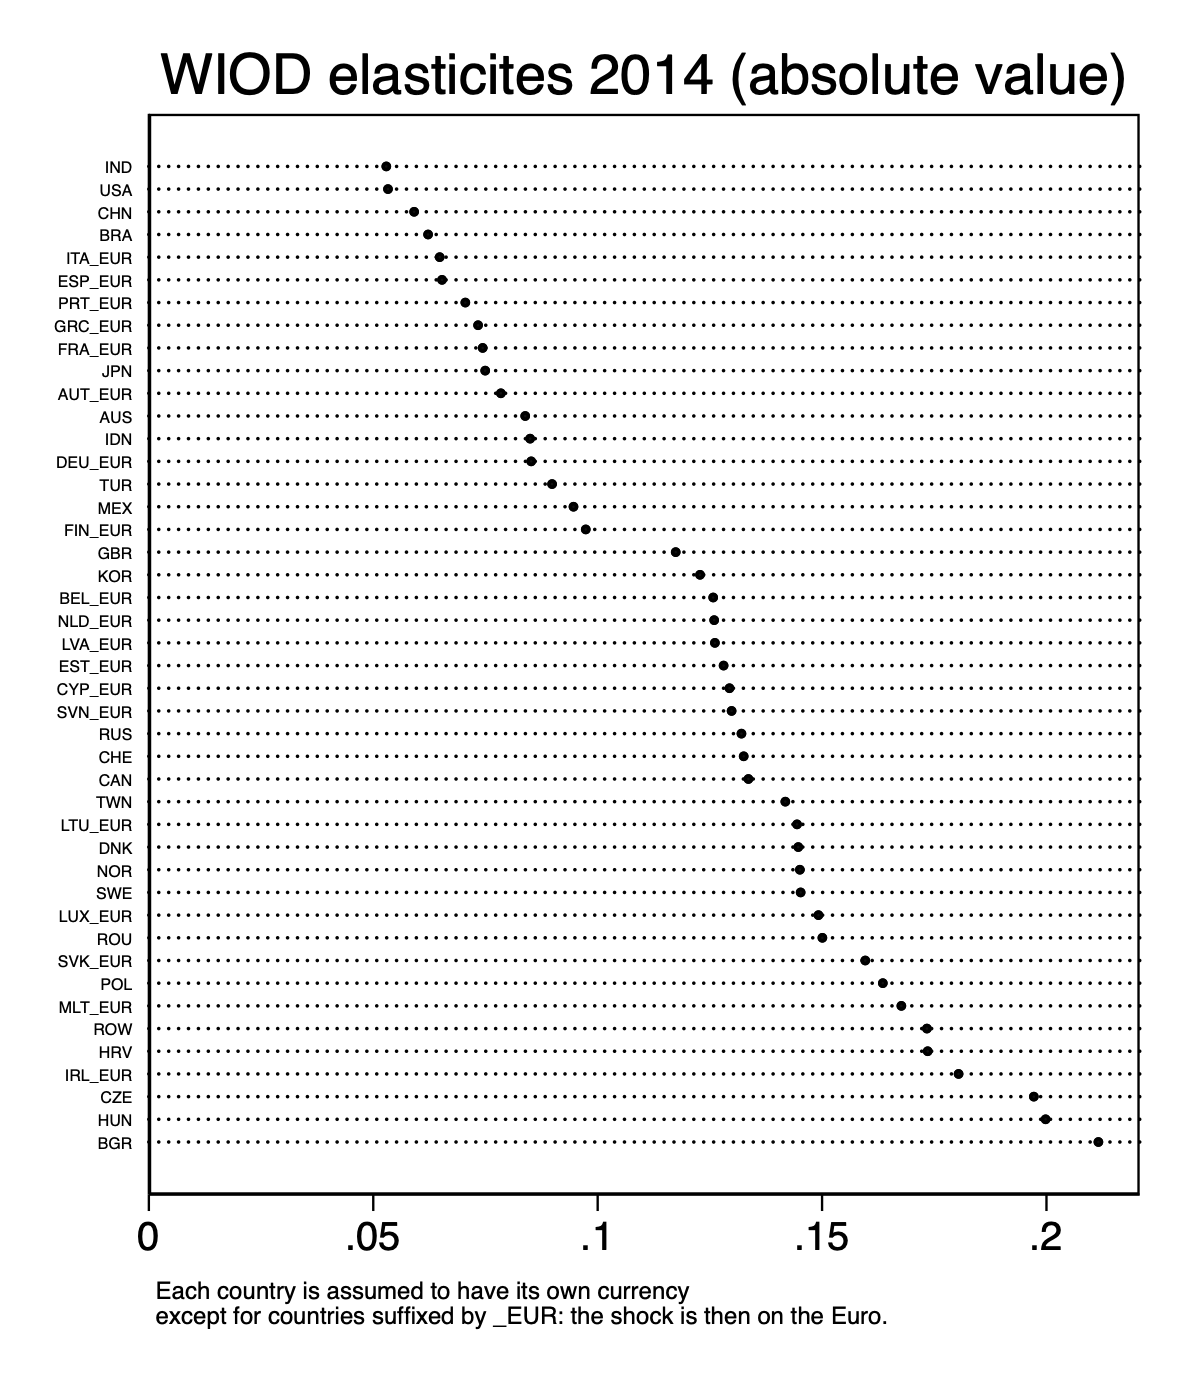
\includegraphics[width=4.5in, height=5.25in]
		{WIOD_HC_elasticities.png}\\
		\floatfoot{Sources: WIOD and authors’ calculations.}
	\end{tabular}
	\label{fig:WIOD_HC_elasticities}
\end{figure}

%This heterogeneity adds to the challenges faced by the European Central Bank when stabilising prices in the monetary union. \\
%VF Spring 2021: je retire la reference a la monnaie ficitive comme convenu 
%For euro-area members, we distinguish between the effect of the appreciation of the euro and the effect of the appreciation of a hypothetical national currency. 
%For France, the elasticity of the HCE deflator to an appreciation of the euro is -0.08. 
%The elastiticy of the HCE deflator to an appreciation of an hypothetical French national currency is -0.122. 

Figure \ref{fig:comp_WIOD_TIVA} compares the results obtained with WIOD and two distinct releases of TiVA for years 2011 and 2014.
\begin{figure}[H]
\centering
\caption{\footnotesize{\textbf{Comparison of the HCE deflator elasticity to the exchange rate for WIOD, TIVA rev. 3 and TIVA rev. 4 (2011 and 2014)}}}
\begin{tabular}{c}
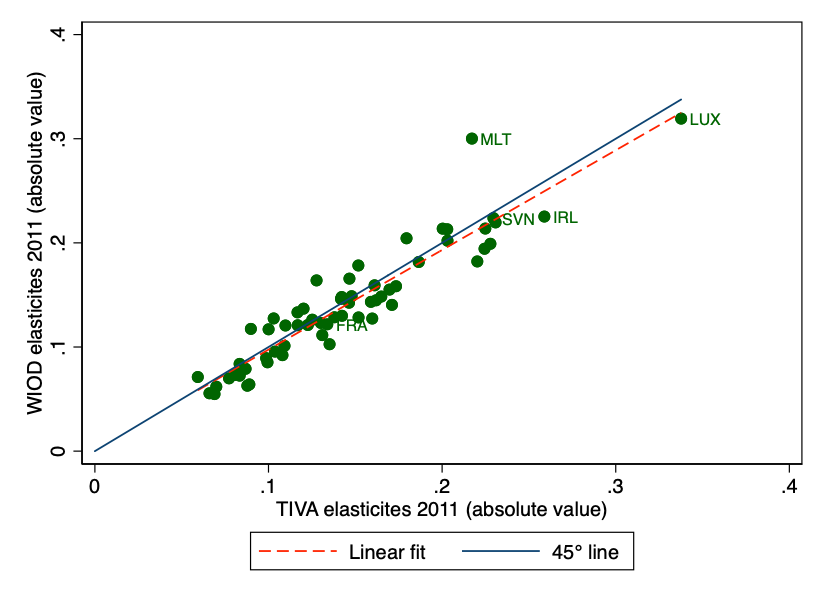
\includegraphics[width=3in, height=2in]{Comparaison_WIOD_TIVA_2011.png}
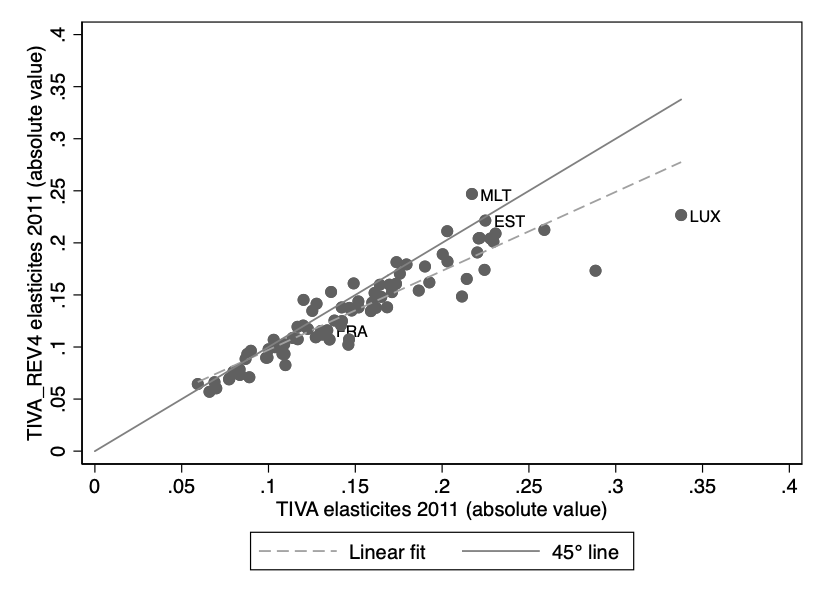
\includegraphics[width=3in, height=2in]{Comparaison_TIVA_REV4_TIVA_2011.png}\\
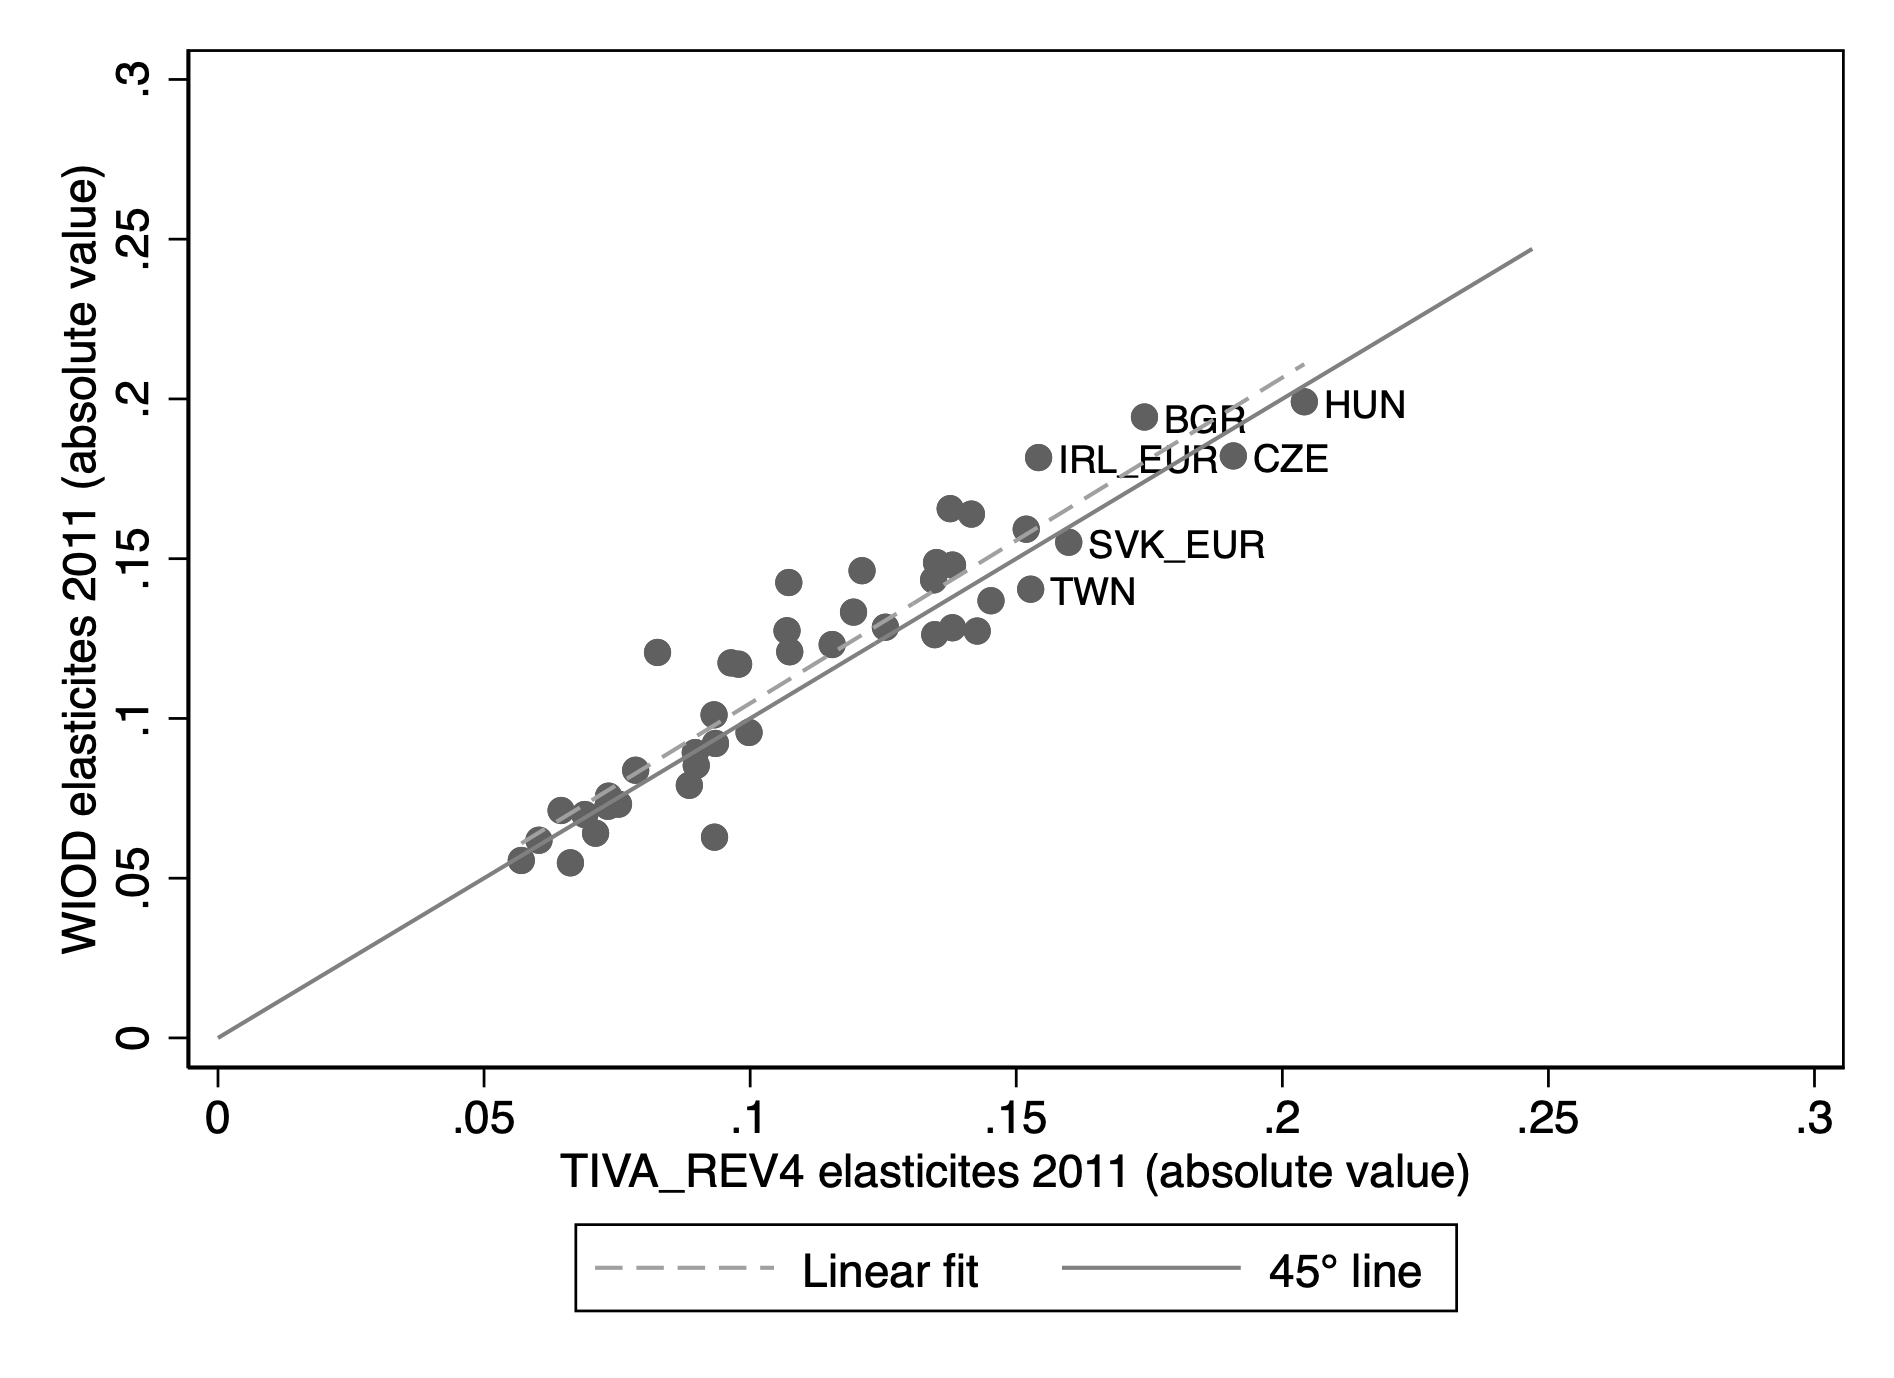
\includegraphics[width=3in, height=2in]{Comparaison_WIOD_TIVA_REV4_2011.png}
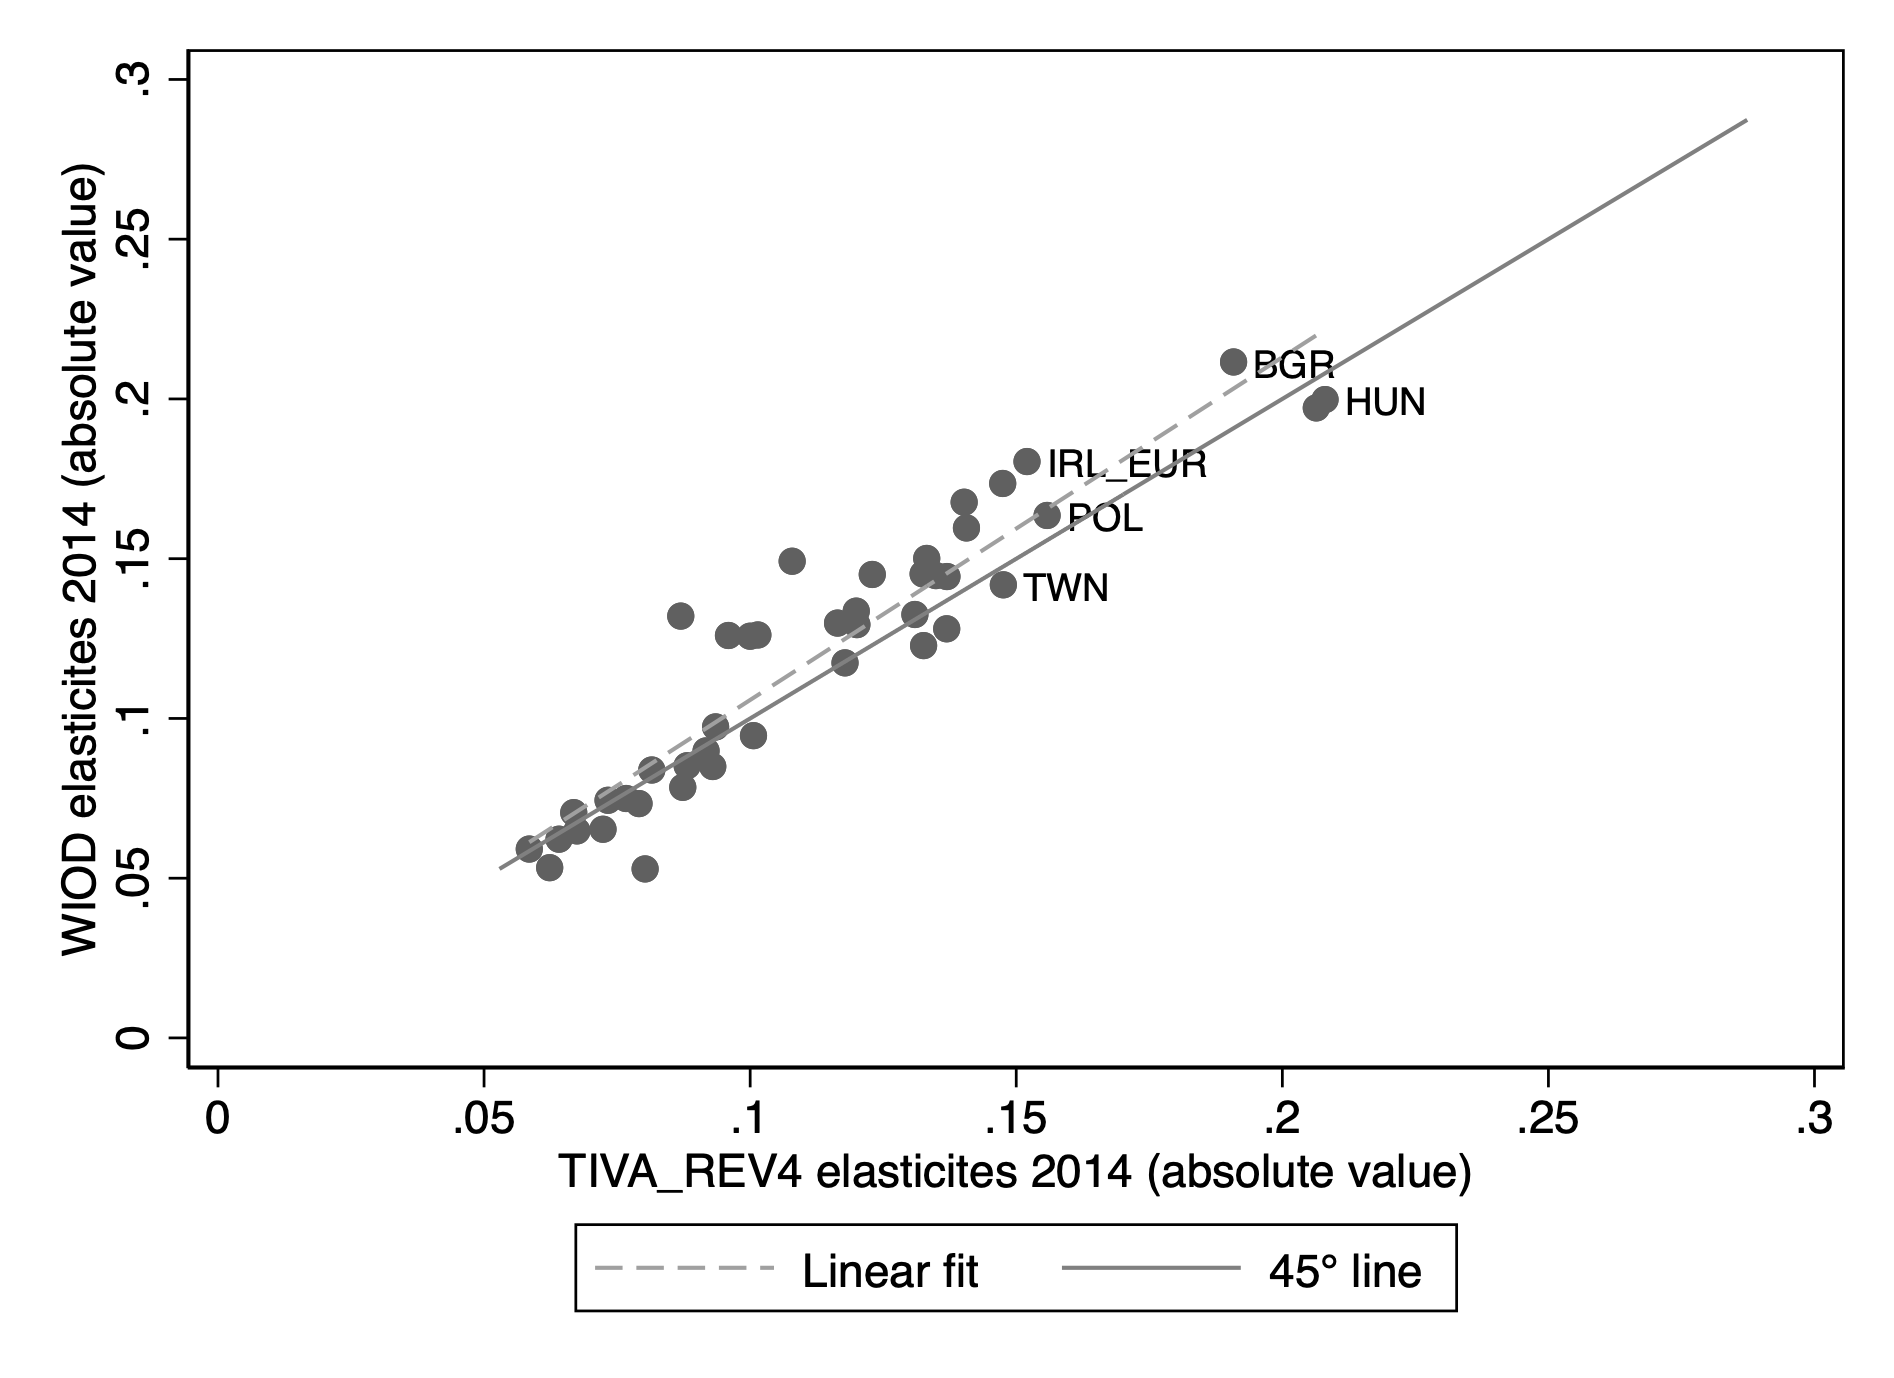
\includegraphics[width=3in, height=2in]{Comparaison_WIOD_TIVA_REV4_2014.png}\\
\floatfoot{Sources: WIOD, TIVA rev. 3 and TIVA rev. 4, authors’ calculations}.
\end{tabular}
\label{fig:comp_WIOD_TIVA}
\end{figure}

Figure \ref{fig:WIOD_HC_E1HC} shows that the value of the elasticity is closely, but not perfectly, related to the share of imported goods and services (from outside the euro area for euro area countries) in household consumption.
The higher the country's import share in consumption, the higher the elasticity of the HCE deflator to the exchange rate. 
We come back to the relations between the HCE deflator and various openness measures in section \ref{sec:extrapo}.
%Small open economies in the euro area post higher import content of consumption. 
%Our findings concur with the literature. For instance, \cite{Ortega2020} find that the direct and indirect import content in consumption %ranges from 12\% in Italy to 33\% in Ireland and Malta, according to calculations based on input-output tables from WIOD.\\

\begin{figure}[H]
	\centering
	\caption{\footnotesize{\textbf{HCE deflator elasticity and share of imported consumption in total consumption (WIOD, 2014)}}}
	\begin{tabular}{c}
		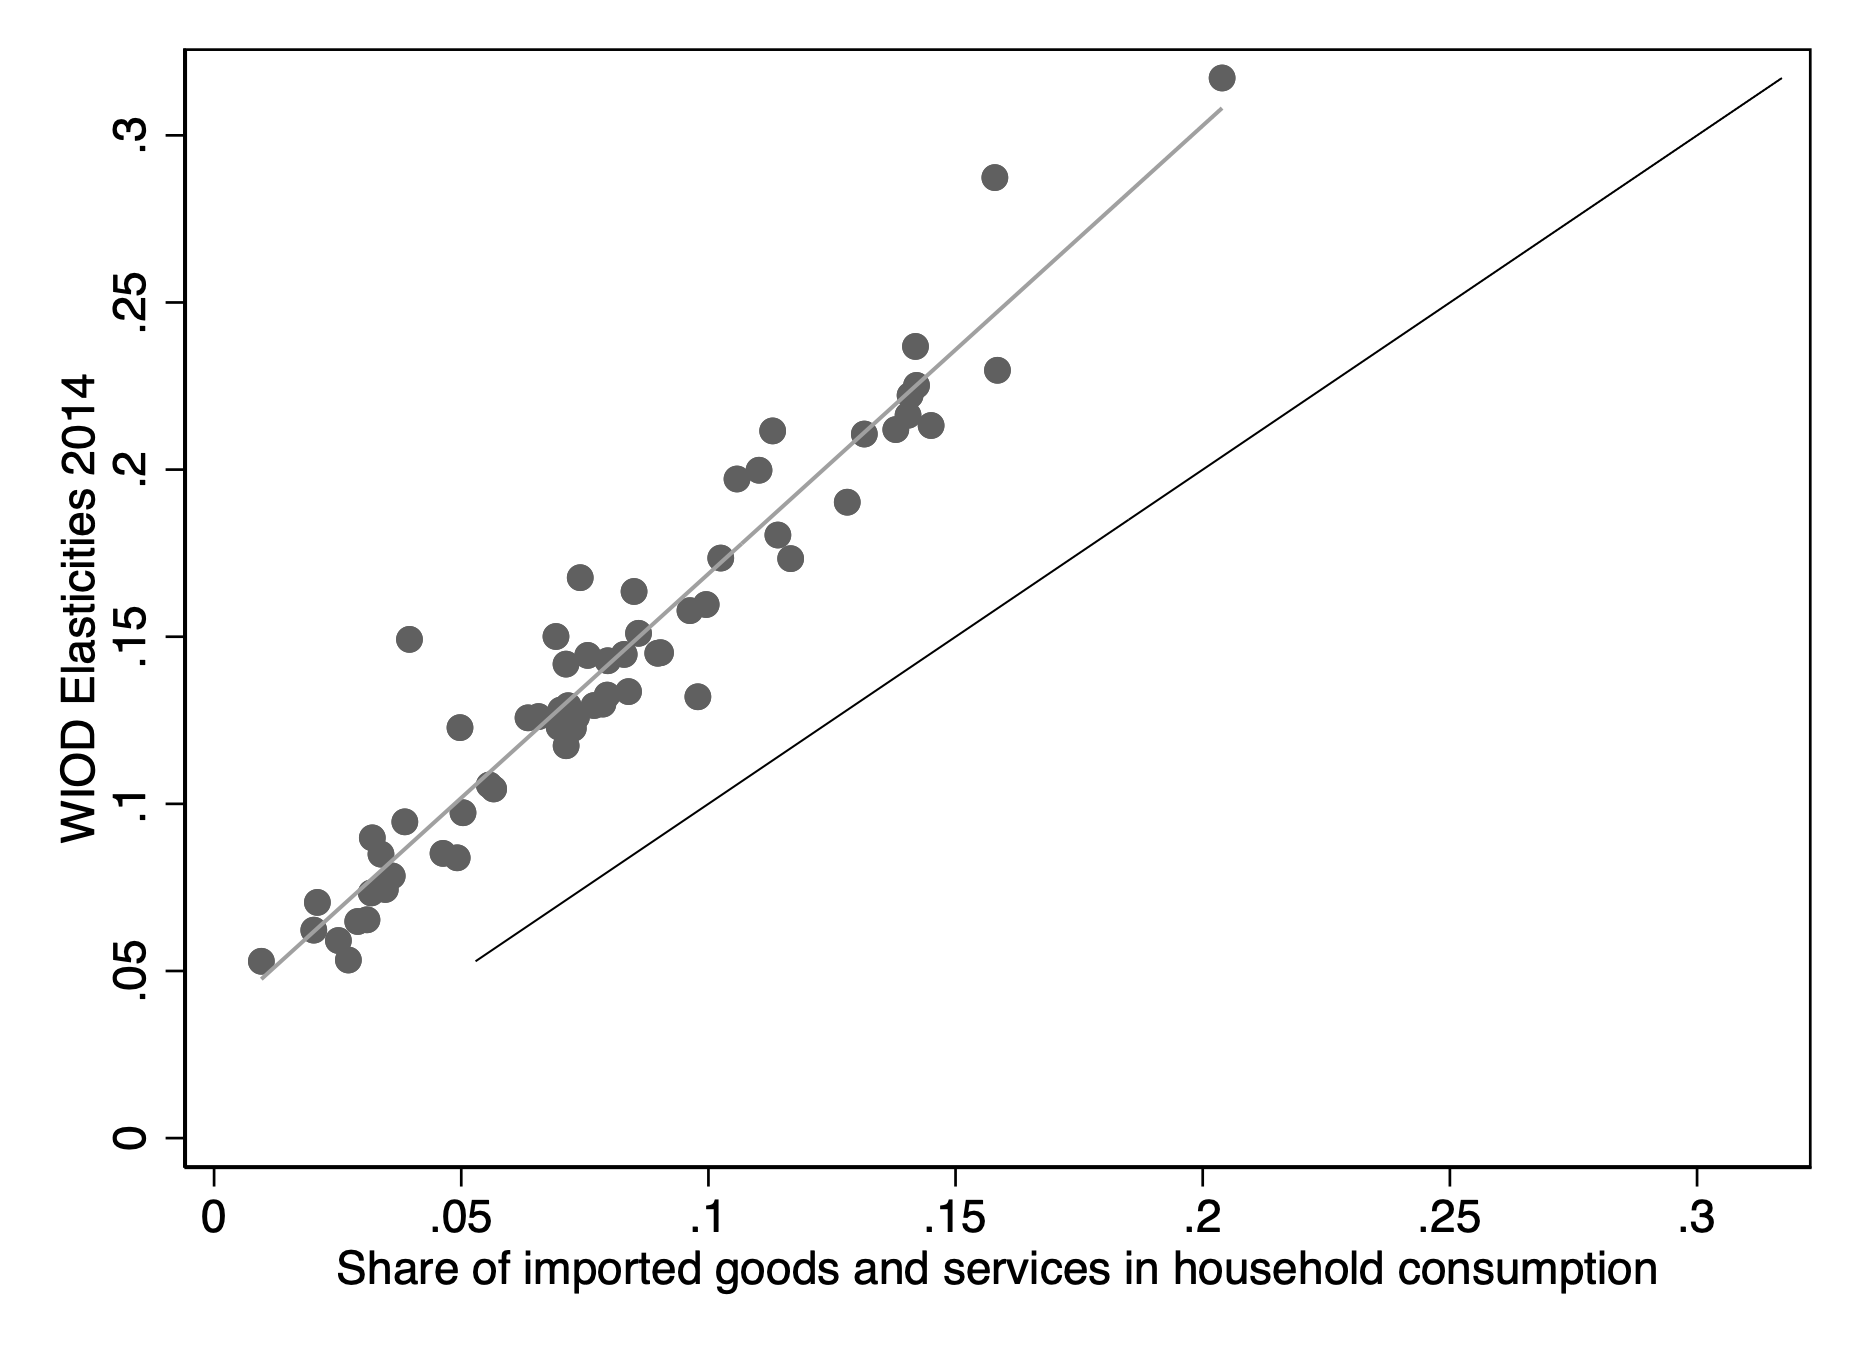
\includegraphics[width=5.0in, height=3.9in]{Comp_s_E1HC_2014_WIOD_HC.png}\\
	\end{tabular}
	\label{fig:WIOD_HC_E1HC}
	\floatfoot{Sources: WIOD and authors’ calculations}
\end{figure}


\subsection{Impact of an appreciation of the US dollar}\label{subsec:usdelasticity}
The model can also track the effect on the domestic economy of variations in the currency of foreign countries.
As an example, we estimate the impact of an appreciation of the US dollar (USD) using WIOD.
This exercise assumes that exports are always invoiced in the exporter’s currency.
We do not take into account the large role of the dollar in international trade invoicing.\\
The US example illustrates that countries are affected in proportion to their trading links with the country whose currency appreciates.
We obtain the highest elasticities for the major trading partners of the US. 
The elasticity of the HCE deflator to the USD amounts to 0.12 for Canada and 0.09 for Mexico (see Figure \ref{fig:WIOD_HC_elasticities_USD}).
The elasticity is below 0.06 for most euro area countries.
Ireland stands out, with an elasticity of 0.09, i.e. close to that of Canada and Mexico. 
The U.S. is Ireland's major trading partner outside of the EU, even if a large portion of Irish imports from the US (pharmaceuticals and aircraft) are later exported by Irish-based firms without being purchased by Irish consumers \citep{Reddan2017}, and therefore have a negligible contribution to domestic consumer goods inflation.
%According to the Irish Central Statistics Office, the U.S. accounted for 19\% of the total current account outflows in 2018, the largest share of any other EU country 

\begin{figure}[H]
	\centering
	\caption{\footnotesize{\textbf{Elasticity of the HCE deflator to the USD (WIOD) - 2014.}}}
	\begin{tabular}{c}
		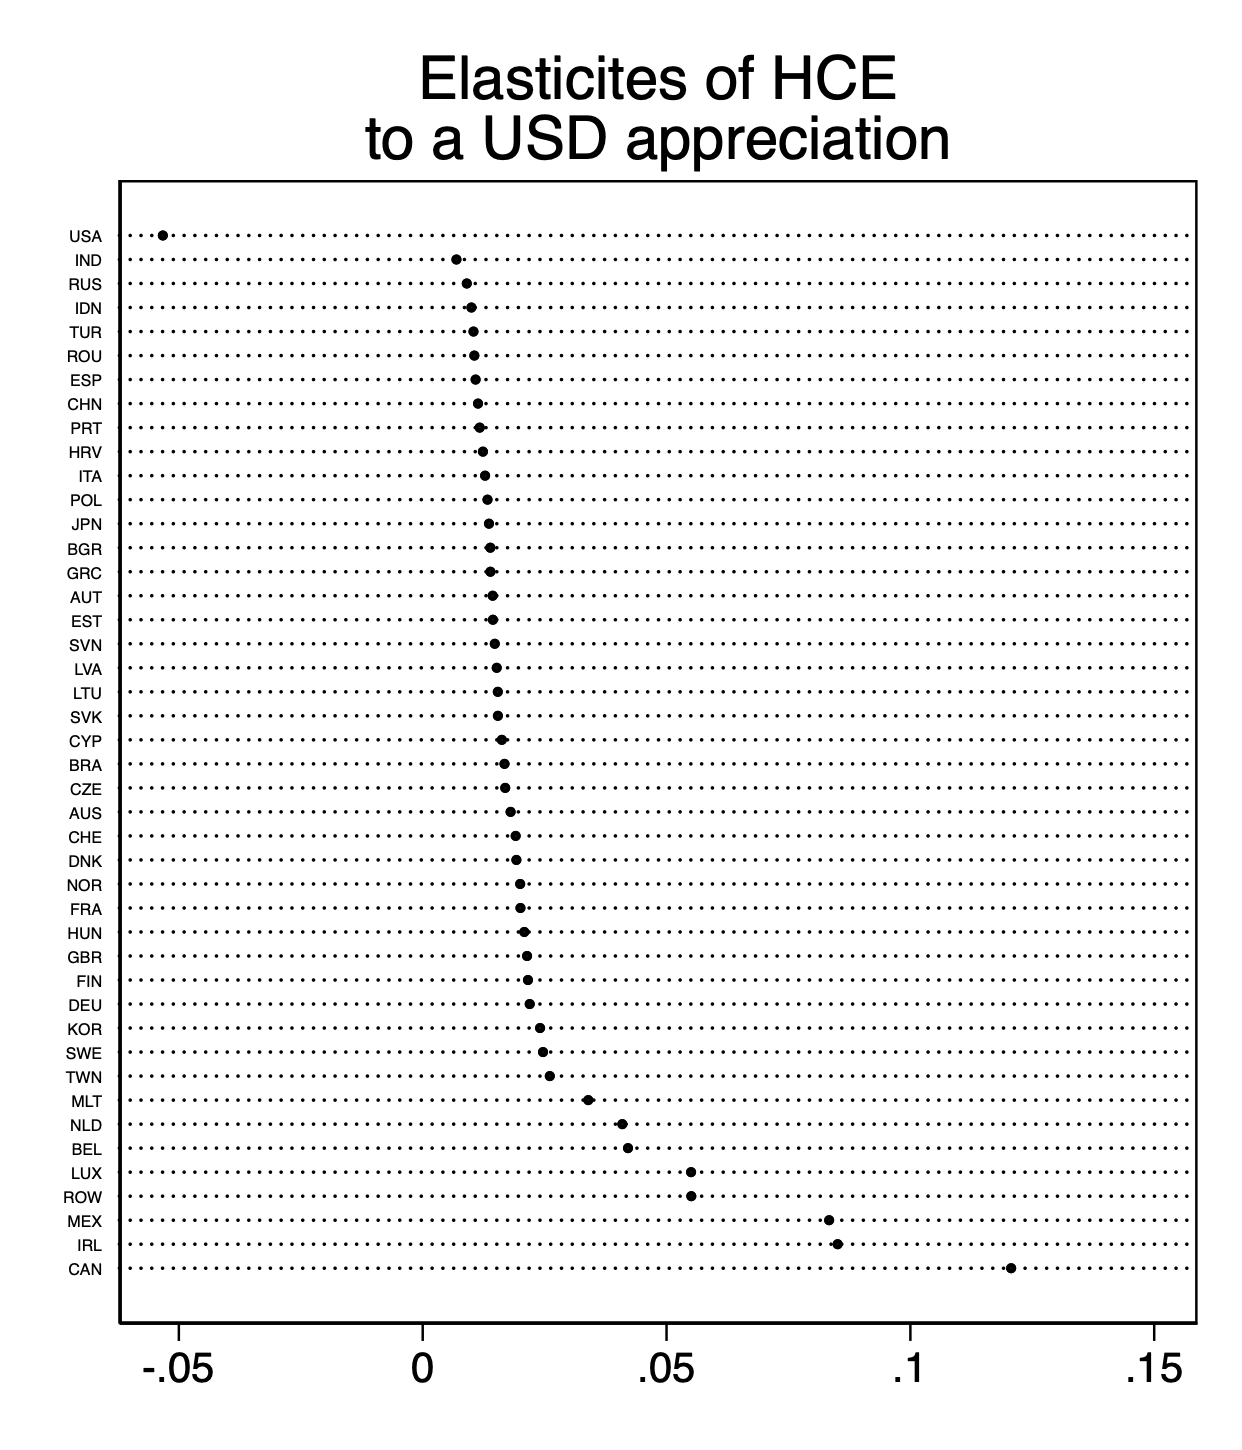
\includegraphics[width=4.5in, height=5.25in]
		{WIOD_HC_elasticities_dollar_appreciation.png}\\
		\floatfoot{Sources: WIOD and authors’ calculations.}
	\end{tabular}
	\label{fig:WIOD_HC_elasticities_USD}
\end{figure}

\subsection{Evolution over time of the HCE deflator elasticity}\label{subsec:timeevol}
The output-weighted elasticity of the HCE deflator to the exchange rate has remained broadly stable over the past two decades.
Output-weighted elasticities are lower than arithmetic means, reflecting the fact that large countries are relatively closed compared to small economies.
Using WIOD, we find that the mean output-weighted elasticity of the HCE deflator increased from 0.06 in 2000 to 0.08 in 2008 (see Figure \ref{fig:PIWIM_LONGITUDINAL}). 
After peaking in 2008, the elasticity sharply declined in 2009. It has hovered around 0.08 in subsequent years. 
Our results concur with the literature.
Using comprehensive measures of global value chain integration, \cite{Timmer2016} find that the expansion of global value chain has slowed down since the Great Recession.\\
While the latest dataset available for WIOD dates back to 2014, MRIO covers the most recent years, up to 2019. 
Results from the MRIO database suggest that the elasticity has bounced back from 2016 onwards, reaching 0.09 in 2019.
However, the version of MRIO we use (March 2021) suffers from data quality issues for 2018 and 2019 (see Online Appendix F). Between 2017 and 2018, the HCE deflator elasticity sharply increased in a number of countries (e.g. China and India). 
%\footnote{For instance, we observe large shifts in the consumption of services in China (see Online Appendix F), suggesting data quality issues in 2018.}
Hence, we assume that the elasticity estimated using MRIO is not reliable for 2018 and 2019 (see Section \ref{sec:Extrapolations} for further details).\\
Overall, our estimates are robust to using different databases.
WIOD and MRIO provide similar elasticities. 
The main difference between the two databases relates to the broader geographic coverage of MRIO, which includes nineteen additional emerging Asian economies. 
Given these economies' relative small size, using MRIO provides aggregate results similar to those of WIOD.
By contrast, using data from TIVA rev. 3, which covers a sample of 64 countries up to 2011, yields a higher elasticity. 
TIVA rev. 3 suggests that the output-weighted elasticity has increased by 25\% between 1995 and 2008, reaching 0.10 in 2008. \\
The higher estimates obtained with TiVA rev. 3 likely reflects the different treatment of contract manufacturing in the 2008 system of national accounts compared to the 1993 system, which reduces imported inputs.
The slight differences observed between WIOD and TiVA rev. 4 likely reflect different ways of reconciling national accounts and international trade statistics.


\begin{figure}[H]
	\centering
	\caption{\footnotesize{\textbf{Evolution of the HCE deflator elasticity, 1995-2019}}}
	\begin{tabular}{c}
		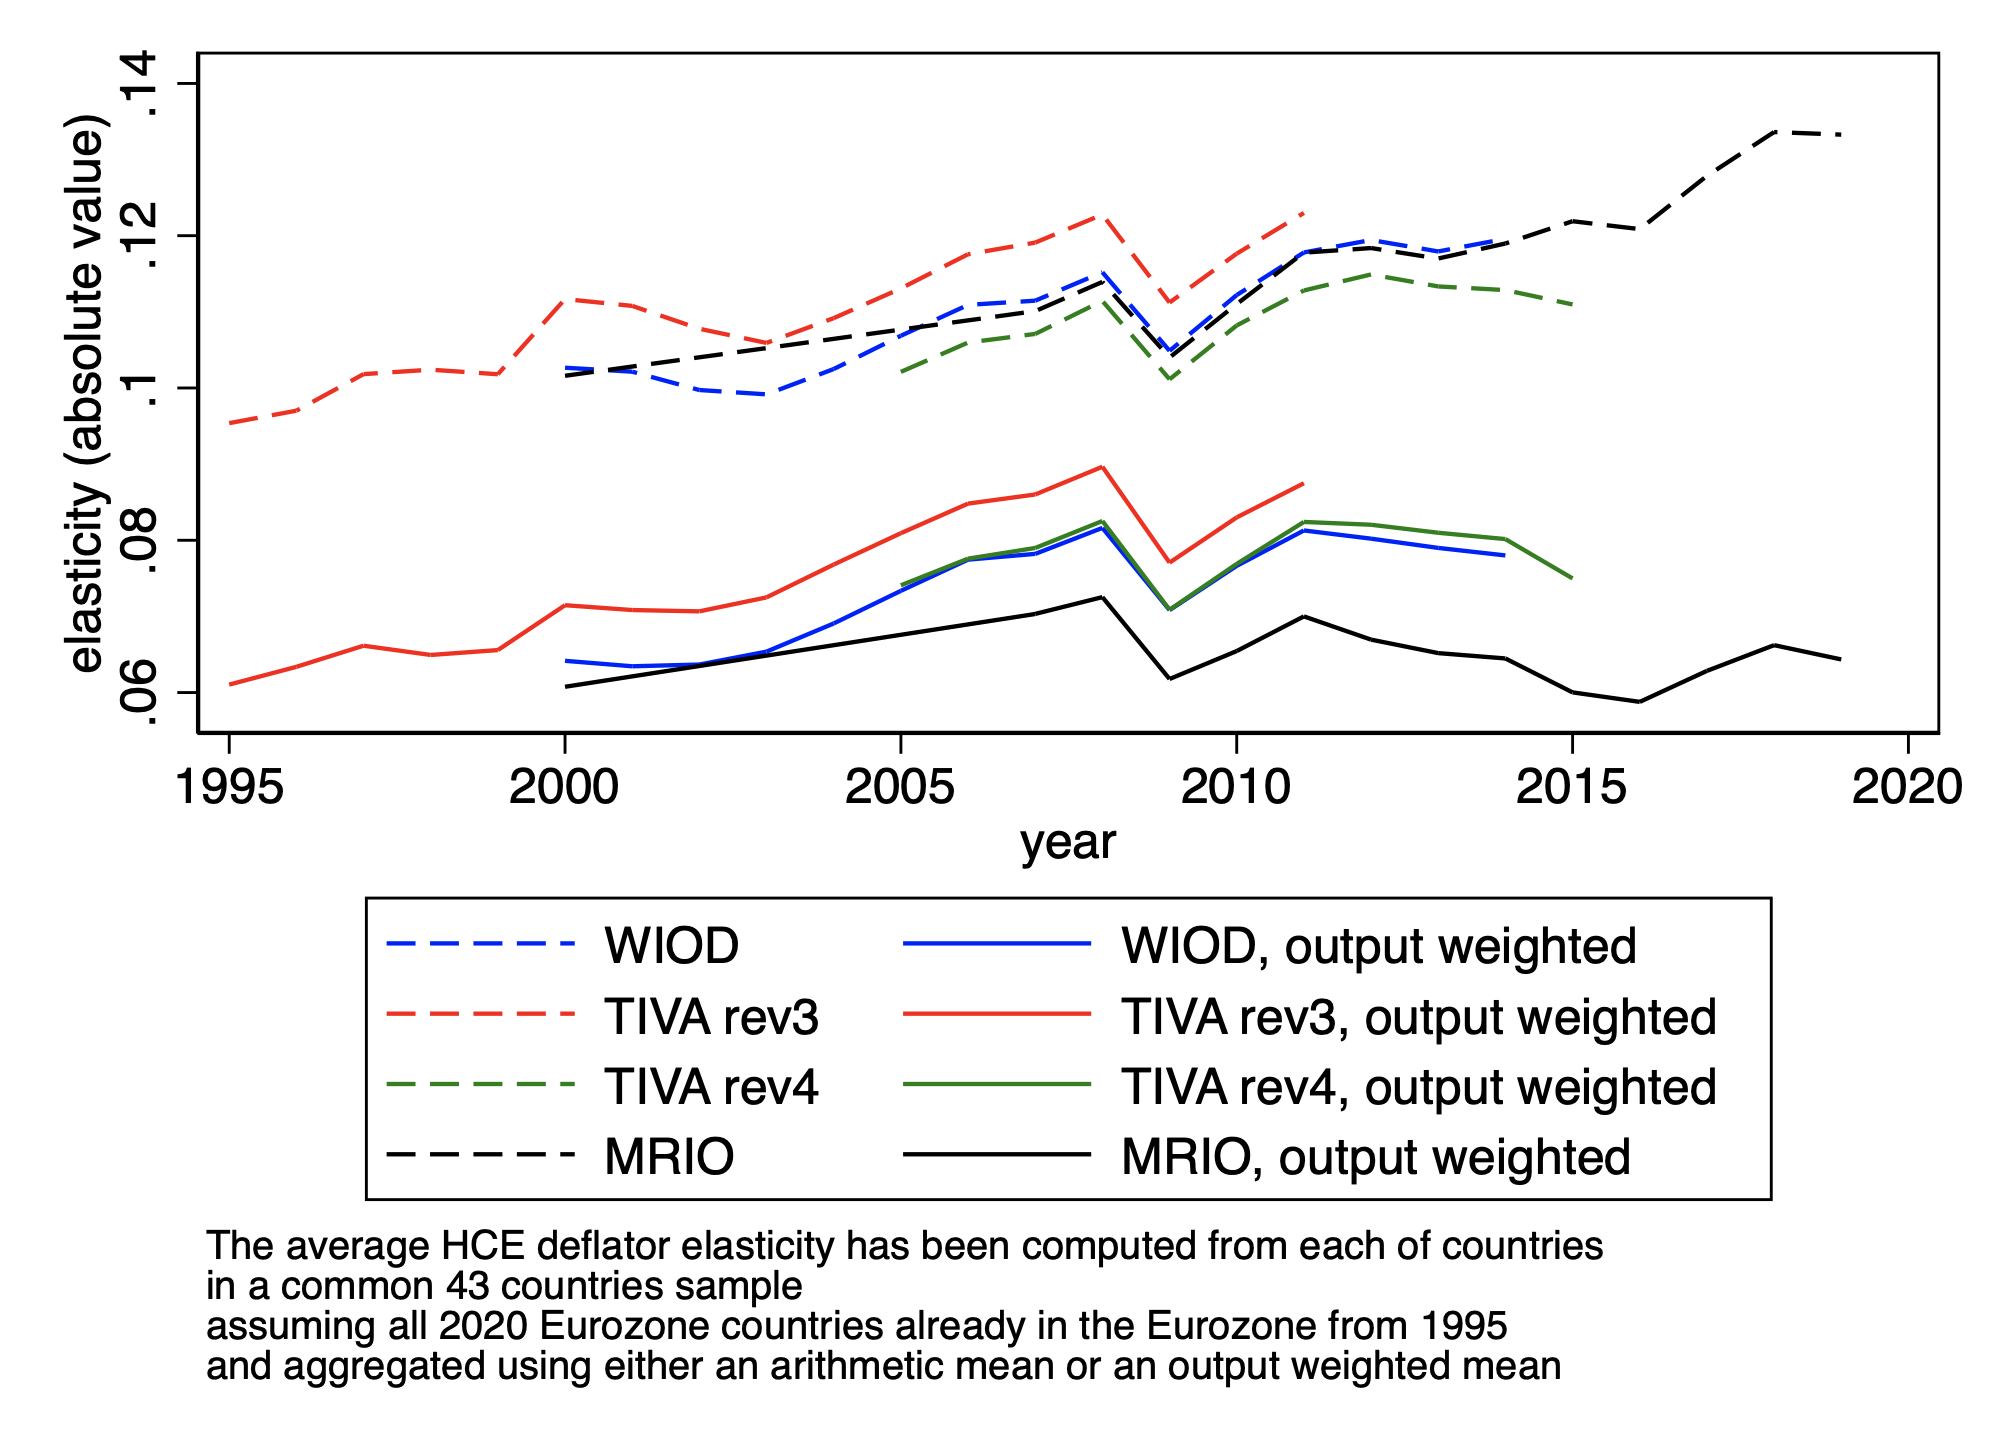
\includegraphics[width=4.5in, height=3in]{PIWIM_LONGITUDINAL.png}\\
		\floatfoot{Sources: WIOD, MRIO, TIVA rev. 3, TIVA rev. 4 and authors’ calculations}
	\end{tabular}
	\label{fig:PIWIM_LONGITUDINAL}
\end{figure}

%
%\begin{figure}[!h]
%	\centering
%	\caption{\footnotesize{\textbf{Consumer price elasticity and share of imported consumption for WIOD 2014}}}
%	\begin{tabular}{c}
%		\includegraphics[width=4.5in, height=3in]
%		{WIOD_HC_E1HC.png}\\
%		\floatfoot{Source: WIOD}.
%	\end{tabular}
%	\label{fig:WIOD_HC_E1HC}
%\end{figure}

\subsection{Contributors to the HCE deflator elasticity}\label{subsec:contributors}
%on ne comprend pas a quoi se referent les cannaux, je suggere d'etre concis 
In this section, we analyse the contributions of each part of the consumption basket to the pass-through of exchange rate variations to consumer prices.
We start with the contributions of domestic versus imported goods.
%Looking at the contribution of different types of goods to $\overline{s_{i}}^{i,HC}$ helps understanding the mechanis at work in PIWIM. One possibility is too look at the predicted effect on domestic goods versus imported goods. 
We define 
\begin{eqnarray}
\overline{s}_i^{i,HC}=\overline{s}_{i,imp}^{i,HC} + \overline{s}_{i,dom}^{i,HC} = S^i.HC^{i,dom}+ S^i.HC^{i,imp}
\label{equ:decomp_impexp}
\end{eqnarray}

Where:
\begin{equation}
\begin{array}{ccccc}
HC^i&=&HC^{i,dom} & + &  HC^{i,imp} \\ 
&=&  \left( \begin{array}{c}
	0 \\
	...\\
	\frac{{hc}_{ij}^i}{hc^i}\\
	...\\
	0
	 \end{array}
	 \right)
&+&
\left( 	\begin{array}{c} \frac{{hc}_{11}^i}{hc^i} \\	...\\0\\...\\\frac{{hc}_{IJ}^i}{hc^i}\end{array}\right) 
\end{array}
\end{equation}

For example,
\begin{equation}
\overline{s}_{i,imp}^{i,HC} = \underset{\begin{subarray}{c}j=1 \dots J   \\ k=1 \dots I \\ k \neq i \end{subarray}}{\mathop \sum}\,{{s}_{kj}^i}.\frac{{hc}_{kj}^i}{hc^i}
\label{equ:share_of_imported}
 \end{equation}


Figure \ref{fig:decomp_origine} shows that changes in the prices of imported final consumer goods and services contribute more to the total effect than changes in the prices of domestic final goods and services.
Furthermore, imported final consumer goods also explain the differences in price elasticities observed between open and relatively closed economies.
Although imported final consumer goods account for a smaller share of total consumption than domestic goods, they are the most impacted by exchange rate fluctuations.\\


\begin{figure}[H]
	\centering
	\caption{\footnotesize{\textbf{Contribution of imported and domestic final goods and services to the HCE deflator elasticity (WIOD, 2014)}}}
	\begin{tabular}{c}
		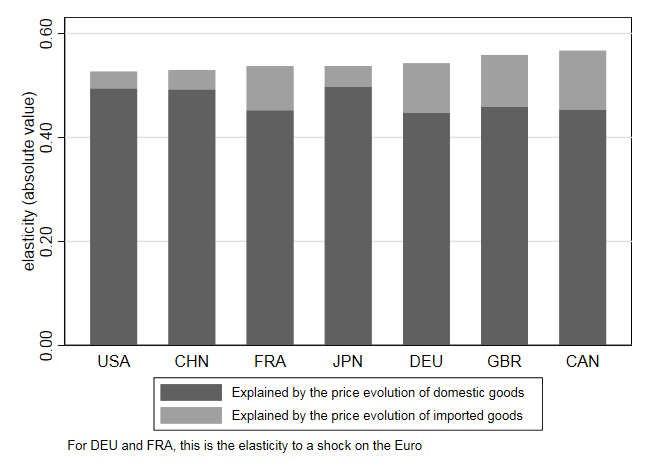
\includegraphics[width=4.5in, height=3in]
		{decomp_origine_WIOD_2014.png}\\
		\floatfoot{Sources: WIOD and authors’ calculations}.
	\end{tabular}
	\label{fig:decomp_origine}
\end{figure}

We also examine the contributions of each sectors to the HCE deflator elasticity.
We regroup industries into four categories: manufacturing goods, services, food and energy. 
Figure \ref{fig:decomp_sect} shows the impact of a change in the exchange rate on the main components of the HCE deflator.
Non-energy industrial goods explain the bulk of the total impact.
However, services also play a significant role, especially in advanced economies. 
Although services are mainly produced domestically and do not rely much on imported inputs, they represent a substantial share of total consumption: even small price changes have large impacts on the HCE deflator. \\ 
Finally, mixing both the industrial and origin analysis shows that domestic core inflation (i.e. all domestic products except food and energy) accounts for a significant share of the total impact (Figure \ref{fig:decomp_sectxorigin}), reflecting the weight of domestic services and non-energy industrial goods in total consumption.
% title Figure 5: contribution of imported and domestic final goods and services to the CPI elasticity to an exchange rate shock
% title Figure 6: contribution of different products to the CPI elasticity to an exchange rate shock
%A major part of the shock comes from lower prices for service consumption (Figure \ref{fig:decomp_sect}). This is paradoxical since, on the one hand, services are not imported a lot and, on the other hand, domestic services do not use many imported inputs. Similarly, domestic core inflation accounts for most of the shock effect for the same reason (Figure \ref{fig:decomp_sectxorigin}). These two phenomena can be explained by the significant weight in the consumption of services on the one hand and domestic services and non-energy industrial goods on the other hand.



\begin{figure}[H]
	\centering
	\caption{\footnotesize{\textbf{Contribution of different products to the HCE deflator elasticity (WIOD, 2014)}}}
	\begin{tabular}{c}
		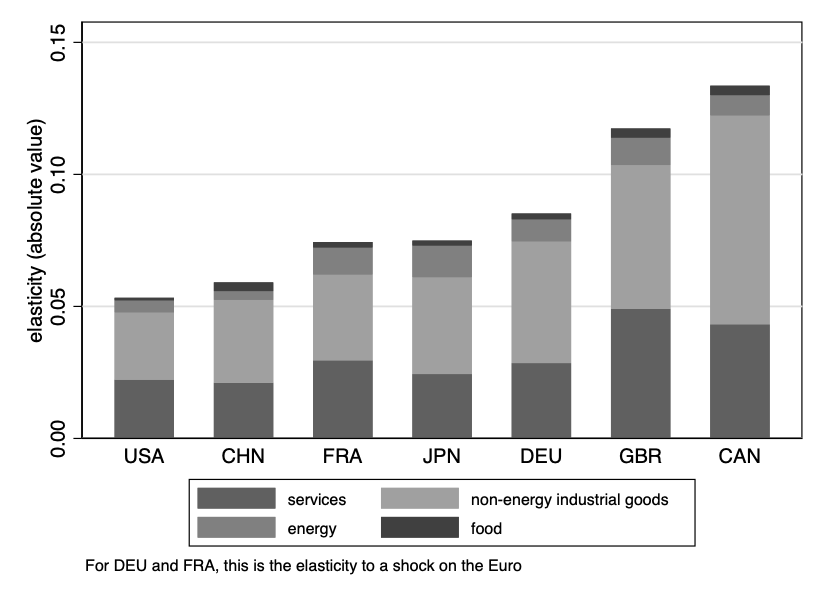
\includegraphics[width=4.5in, height=3in]
		{decomp_sect.png}\\.
	\end{tabular}
	\floatfoot{Sources: WIOD and authors’ calculations}
	\label{fig:decomp_sect}
\end{figure}



\begin{figure}[H]
	\centering
	\caption{\footnotesize{\textbf{Contribution of domestic and imported components to the HCE deflator elasticity (WIOD, 2014)}}}
	\begin{tabular}{c}
		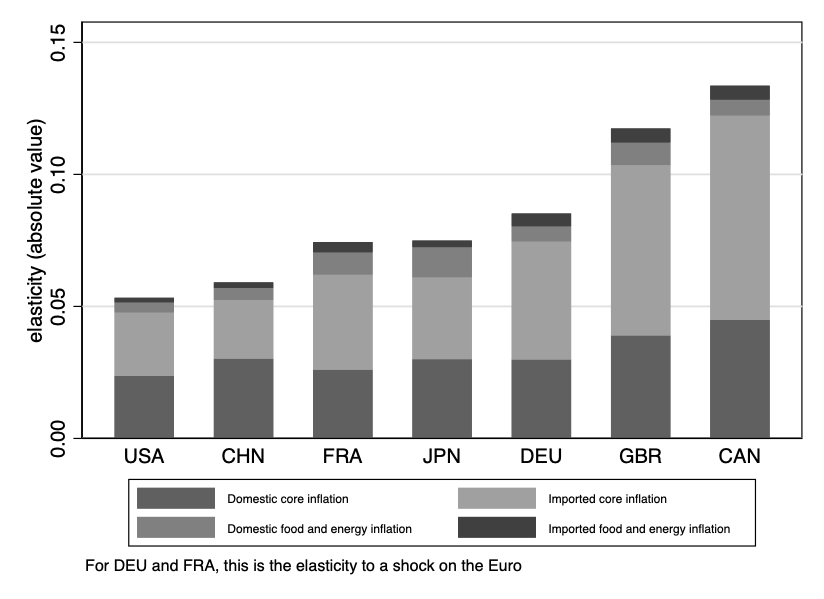
\includegraphics[width=4.5in, height=3in]
		{decomp_sectxorigin.png}\\
		\floatfoot{Sources: WIOD and authors’s calculations}.
	\end{tabular}
	\label{fig:decomp_sectxorigin}
\end{figure}




%
%We can then define the contribution of imported consumption goods to an exchange rate shock as $\nicefrac{\overline{s}_{i,imp}^{i,HC}}{\overline{s}_{i}^{i,HC}} = \nicefrac{S^i.HC^{i,imp}}{S^i.HC^{i}}$. We can also define the sensitivity of imported consumption prices as $ \frac{\nicefrac{S^i.HC^{i,imp}}{S^i.HC^{i}}}{\vec{1}.HC^i,imp}$ where $\vec 1$ is a horizontal vector of ones.
%For example, if an appreciation exchange rate reduce household consumption prices by 20\%, that household consumption is 50\% imported and that imported consumption goods prices evolution cause in a reduction of household consumption prices of 15\%, then the contribution of imported consumption goods will be 0.75 (=.15/.20)and their sensitivity of 1.5 (=0.75/0.5).
%
%GD : PEUT-ÊTRE Y A-T-IL UNE MANIÈRE DE SIMPLIFIER L'EXPRESSION DE LA SENSITIVITÉ, MAIS JE NE VOIS PAS COMMENT FAIRE...
%
%Figure \ref{fig:share_impt} shows, for example, that the contribution of imported consumption is higher than 0.5 in most countries. While imported consumption has a smaller share in total consumption, this is over-compensated by the sensitivity of its prices to exchange rate shocks, as show by the comparison of \ref{fig:intensity_dom} and \ref{fig:intensity_impt}.
%
%Similar decompositions of the matrix $HC^i$ can be done to analyse the contribution of different sectors. decompose the effect between sectors. That allows the identification of the contribution of different sectors to the inflation shocks in different countries.
%Figure \ref{fig:share_sector} shows that non-energy industrial goods and services have the highest contribution. Energy is highly sensitive to exchange rate shocks (see \ref{fig:intensity_dom} and \ref{fig:intensity_impt}), but its share in consumption is too small for its contribution to the final effect to be large.
%
%
%
%\begin{figure}[p]
%\RawFloats
%\centering
%\caption{\footnotesize{\textbf{Contribution of imported final consumption to the impact of a nominal exchange rate shock (see eq. \ref{equ:share_of_imported})}}}
%\begin{tabular}{c}
%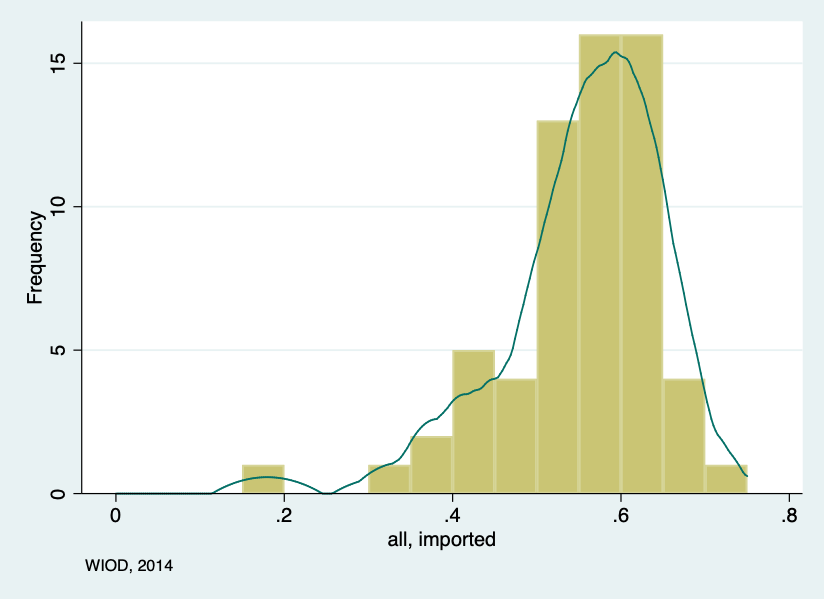
\includegraphics[width=5.0in, height=3.5in]{Share_impt_HC_WIOD_2014.png}\\
%\floatfoot{Interpretation note: the contribution of imported final consumption to the impact of a nominal exchange rate shock is between 55\% and 60\% for 16 countries}
%\end{tabular}
%\label{fig:share_impt}
%
%\caption{\footnotesize{\textbf{Contribution of sector-specific final consumption to the impact of a nominal exchange rate shock}}}
%\begin{tabular}{c}
%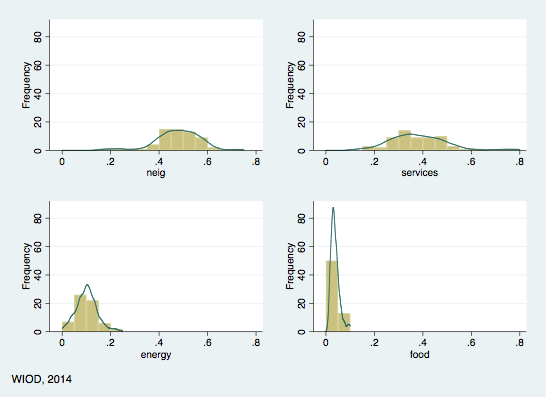
\includegraphics[width=5.0in, height=3.5in]{Share_sector_HC_WIOD_2014.png}\\
%\floatfoot{Interpretation note: the contribution of final energy consumption to the impact of a nominal exchange rate shock is lower than 15\% in most countries}
%\end{tabular}
%\label{fig:share_sector}
%\end{figure}
%
%
%
%
%\begin{figure}[p]
%\RawFloats
%\centering
%\caption{\footnotesize{\textbf{Sensitivity of different domestic sectors to an exchange rate shock}}}
%\begin{tabular}{c}
%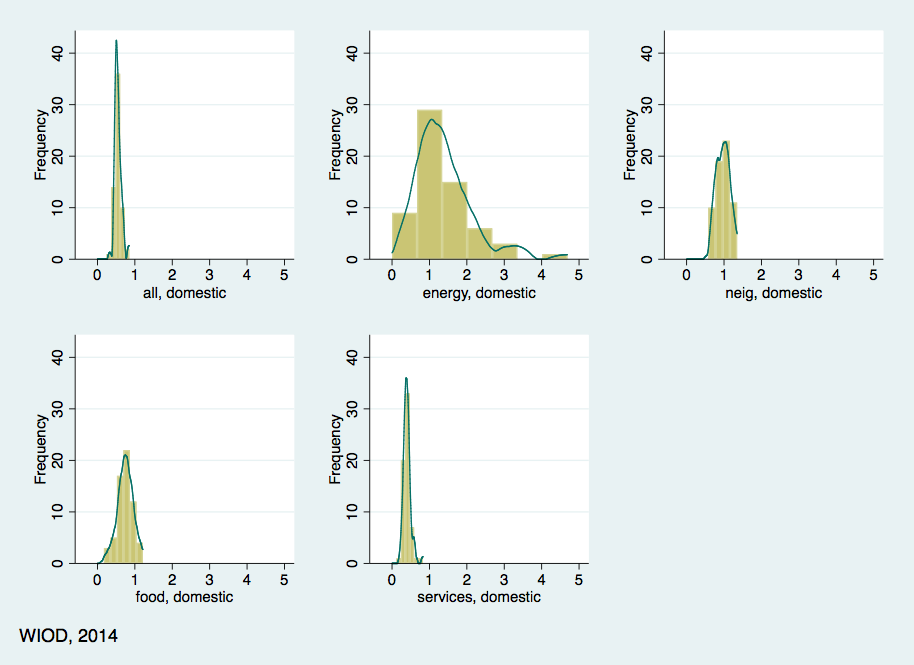
\includegraphics[width=5.0in, height=3.5in]{Int_HC_WIOD_2014_dom.png}\\
%\floatfoot{Intensity is measured as the explained share of inflation change divided by the share in final consumption}
%\end{tabular}
%\label{fig:intensity_dom}
%
%\caption{\footnotesize{\textbf{Sensitivity of imported sectors to an exchange rate shock}}}
%\begin{tabular}{c}
%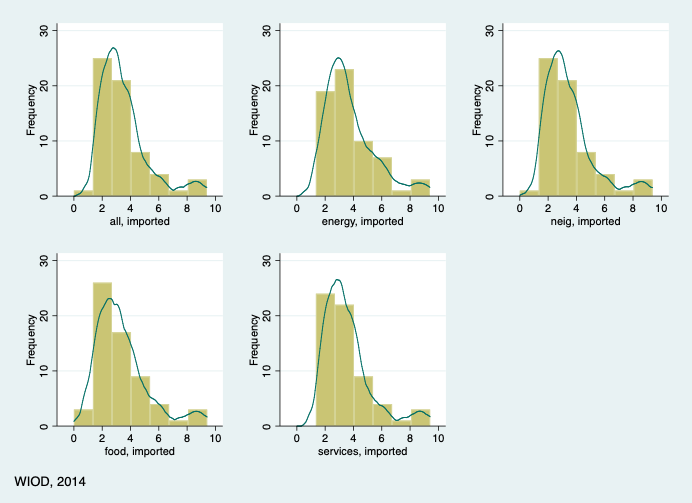
\includegraphics[width=5.0in, height=3.5in]{Int_HC_WIOD_2014_impt.png}\\
%\floatfoot{Intensity is measured as the explained share of inflation change divided by the share in final consumption}
%\end{tabular}
%\label{fig:intensity_impt}
%\end{figure}

\section{Filling the data gap: estimating the HCE deflator elasticity without resorting to WIOTs}
\label{sec:extrapo}
% on ne comprend pas la formulation actuelle sur les canaux, je propose plus explicite
\subsection{Assessing the role of global value chains in the transmission of exchange rate variations to domestic prices}
In this section, we analyse the determinants of the HCE deflator elasticity. 
In particular, we assess the role of global value chains in the transmission of an exchange rate appreciation to the HCE deflator. 
We identify four channels through which an exchange rate appreciation impacts the HCE deflator when production processes are global: \textit{i)} the prices of imported final goods sold directly to domestic consumers;
\textit{ii)} the prices of imported inputs entering domestic production; 
%Hence, a currency appreciation reduces the price of imported inputs, and thus further reduces domestic consumer prices. 
\textit{iii)} the price of exported inputs feeding through imported foreign production;
\textit{iv)}, changes in domestic and foreign production costs in turn passing through to the price of inputs for domestic and foreign goods and causing further changes in production costs through input-output linkages.\\
Mathematically, we break down $\overline{s_{i}}^{i,HC}$ into these different elements.
Starting from equation \ref{eq:eqdomcurrency}, we have:
\begin{equation}
\begin{array}{lccl}
	S^ i&=&C^i	&+ \left(\hat{C}^i_\$.{\cal B}^i+{C^i}{\tilde{{\cal B}^i}}\right)*{{(I-{\cal A})}^{-1}} \\
	S^i &=&\underbrace{C^i}_{\substack{\text{(E1) direct effect through} \\ \text{ imported consumption goods}}}&+ \underbrace{{C^i}{\tilde{{\cal B}^i}}}_{\substack{\text{(E2) effect on} \\ \text{ \emph{domestic} consumption goods} \\ \text{ through \emph{imported} inputs}}}  + \underbrace{\hat{C}^i_\$.{\cal B}^i}_{\substack{\text{(E3)  effect on} \\ \text{\emph{imported} consumption goods} \\ \text{through \emph{domestic} inputs}}} \\ &&+\underbrace {\left( \hat{C}^i_\$.{\cal B}^i + {C^i}{\tilde{{\cal B}^i}}\right)*{{(I-{\cal A})}^{-1}}*{\cal A}}_{\text{(E4) residual}} \\
\end{array}
\label{eq:decomp}
\end{equation}

Defining $HC^{i,dom}$ and $HC^{i,imp}$ as the domestic and imported shares of $HC^i$ and adjusting the dimension of $E1$, $E2$ and $E3$, we have:

\begin{equation}
\begin{array}{lccl}
\overline{s}_{i}^{i,HC}&=S^i.HC^i=E1.HC^i+E2.HC^i+E3.HC^i+E4.HC^i \\
&=E1.HC^{i,imp}+E2.HC^{i,dom}+E3.HC^{i,imp}+E4.HC^i
 \end{array} 
 \label{eq:eqtoto}
 \end{equation}
 
When the domestic currency appreciates, $E1.HC^{i,imp}$ ($E1.HC$ hereafter) and $E2.HC^{i,dom}$ ($E2.HC$ hereafter) reduce consumer prices in country $i$, whereas $E3.HC^{i,imp}$ ($E3.HC$) increases them. 
This decomposition differs from equation \ref{equ:decomp_impexp}. 
Equation \ref{equ:decomp_impexp} focuses on the contribution of domestic versus imported goods to the HCE deflator elasticity to the exchange rate.
By contrast, equation \ref{eq:eqtoto} highlights the transmission channels of the exchange rate fluctuation.
Figure \ref{fig:decompositionofs} plots the shares of $E1.HC$, $E2.HC$, $E3.HC$ and $E4.HC^i$ ($E4.HC$) in $\overline{s}_{i}^{i,HC}$.  
Direct effects through imported consumer goods ($E1.HC$) dominate. 
The effect on domestic consumer goods through imported inputs ($E2.HC$) is also important.
While the effect on imported consumer goods through domestic inputs ($E3.HC$) is negligible (except for Germany and the Netherlands), $E4.HC$ accounts for 10\% to 30\% of $\overline{s}_{i}^{i,HC}$ for most countries (and close to 50\% for India, Brazil, Portugal and Luxembourg). With the exception of Luxembourg, the less open to trade is a country, the larger the share of $E4.HC$. \\
Figure \ref{fig:shareofs} shows that input-output mechanisms (i.e. all channels except $E1.HC$) explain a large share of the elasticity, especially for large countries or euro area countries.
The share explained by input-output mechanisms has increased until 2013-2014 (see Figure \ref{fig:shareofsthroughtime}), implying an increasing need of data from WIOTs to perform our computations.

\begin{figure}[H]
\centering
\caption{\footnotesize{\textbf{Decomposition of $\overline{s}_{i}^{i,HC}$ into $E1.HC$, $E2.HC$, $E3.HC$ and $E4.HC$ (WIOD, 2014)}}}
%La figure vient de Étude rapport D+I et Bouclage Mondial_oil.do
\begin{tabular}{c}
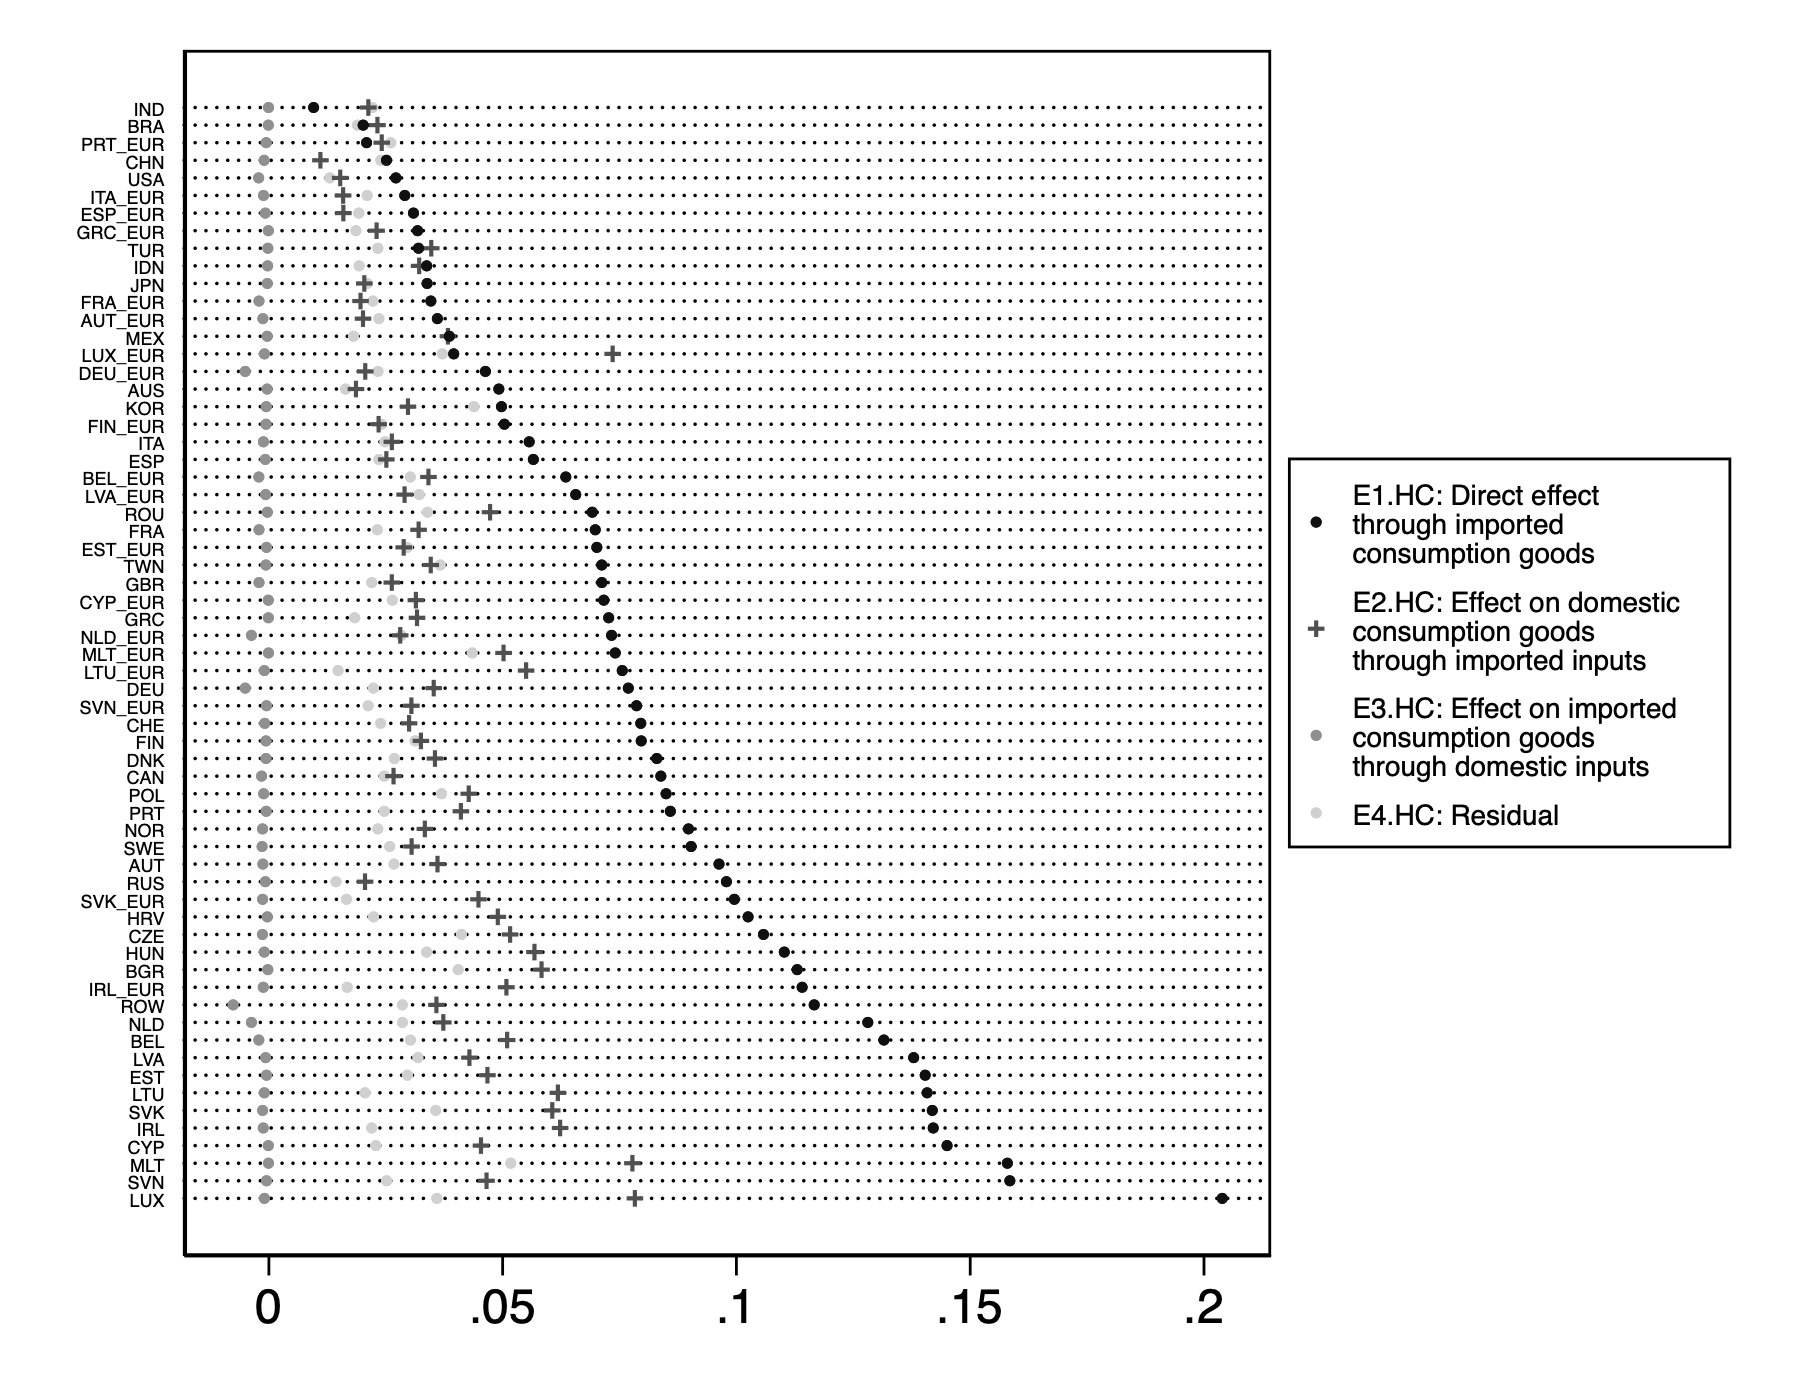
\includegraphics[width=5.0in, height=3.5in]{distribution_components_WIOD_2014.png}\\
\floatfoot{Sources: WIOD and authors’ calculations}. \\
\end{tabular}
\label{fig:decompositionofs}
\end{figure}


\begin{figure}[H]
	\centering
	\caption{\footnotesize{\textbf{Decomposition of $\overline{s}_{i}^{i,HC}$ (WIOD, 2014)}}}
	%La figure vient de Étude rapport D+I et Bouclage Mondial_oil.do
	\begin{tabular}{c}
		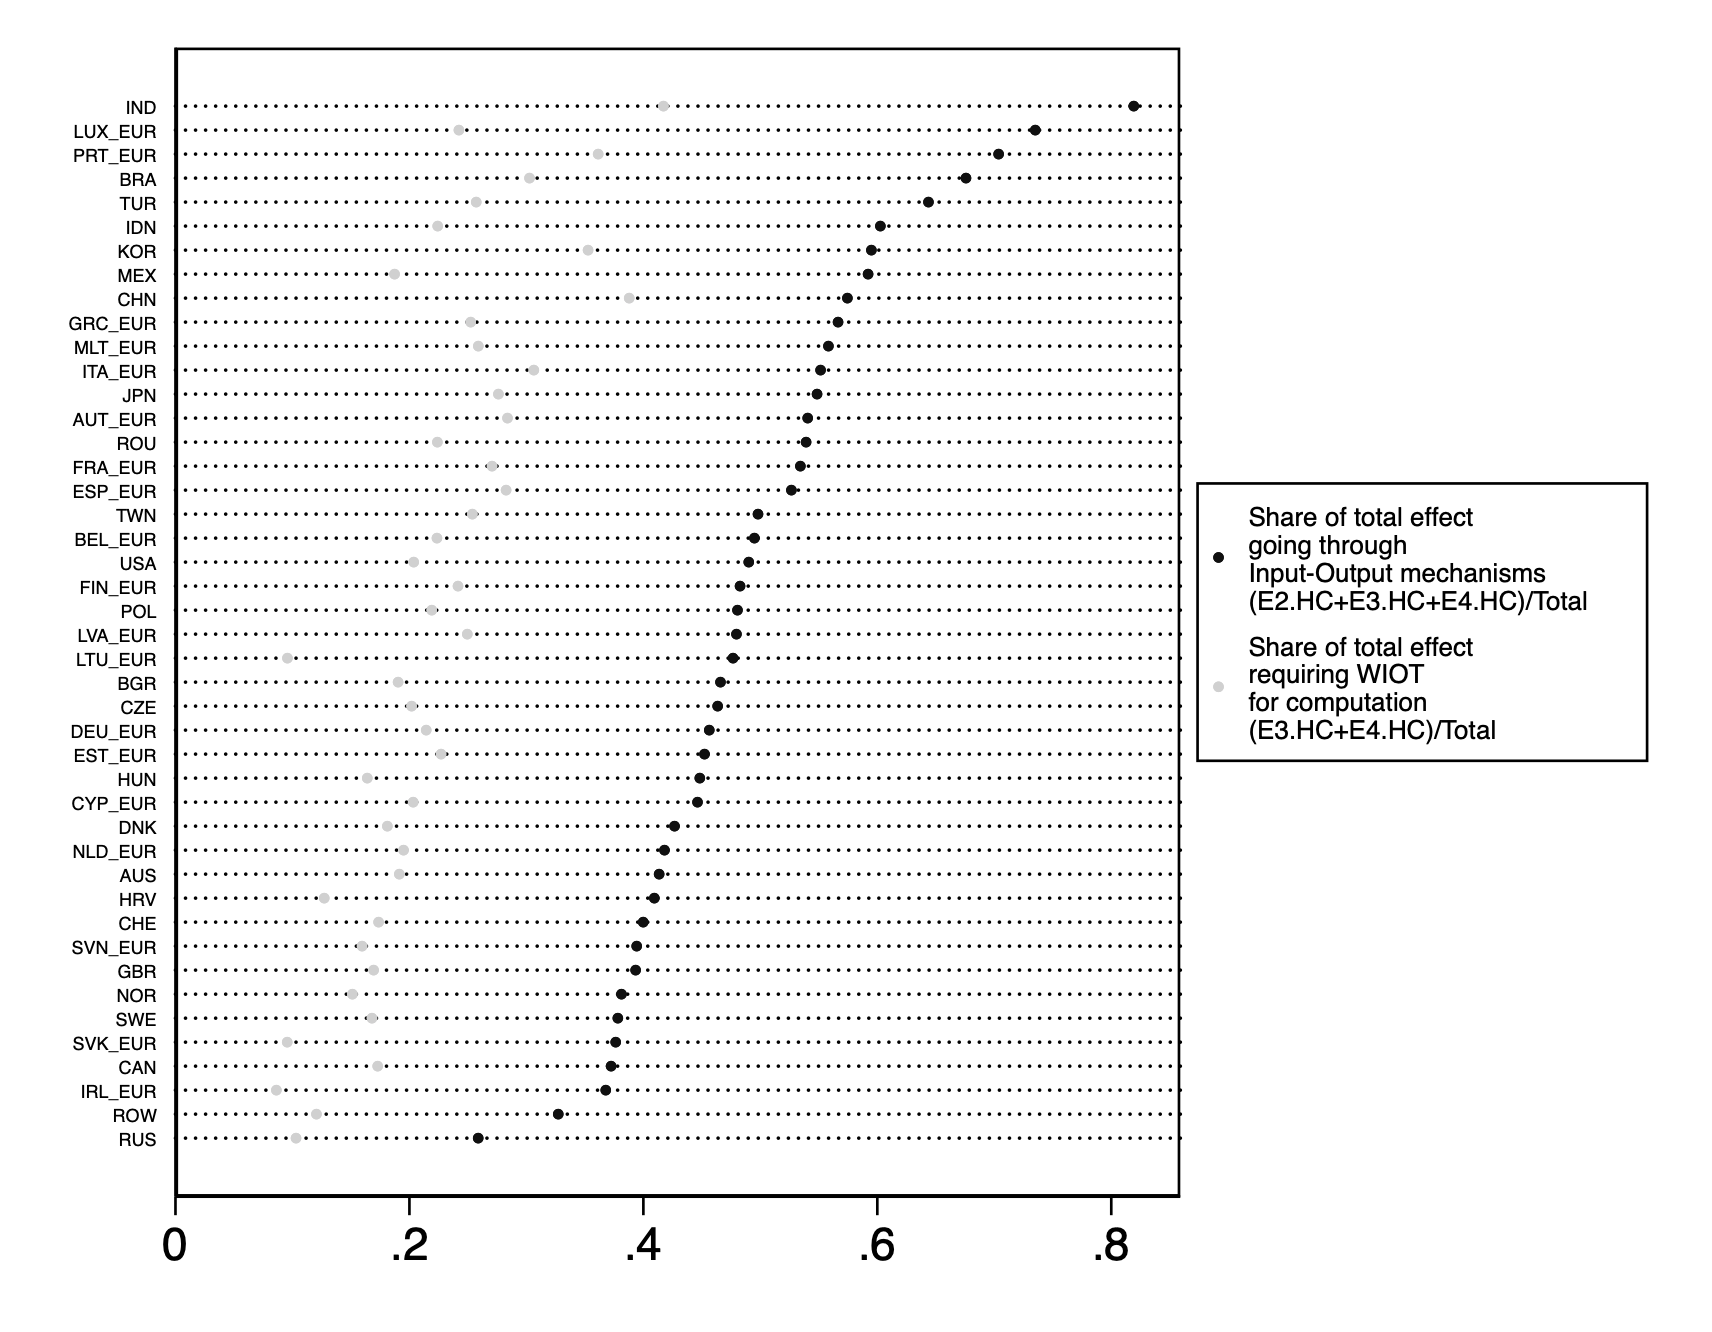
\includegraphics[width=5.0in, height=3.5in]{share_components_WIOD_2014.png}\\
		\floatfoot{Sources: WIOD and authors’ calculations}. \\
	\end{tabular}
	\label{fig:shareofs}
\end{figure}


\begin{figure}[H]
	\centering
	\caption{\footnotesize{\textbf{Decomposition of $\overline{s}_{i}^{i,HC}$ through time}}}
	%La figure vient de Étude rapport D+I et Bouclage Mondial_oil.do
	\begin{tabular}{c}
		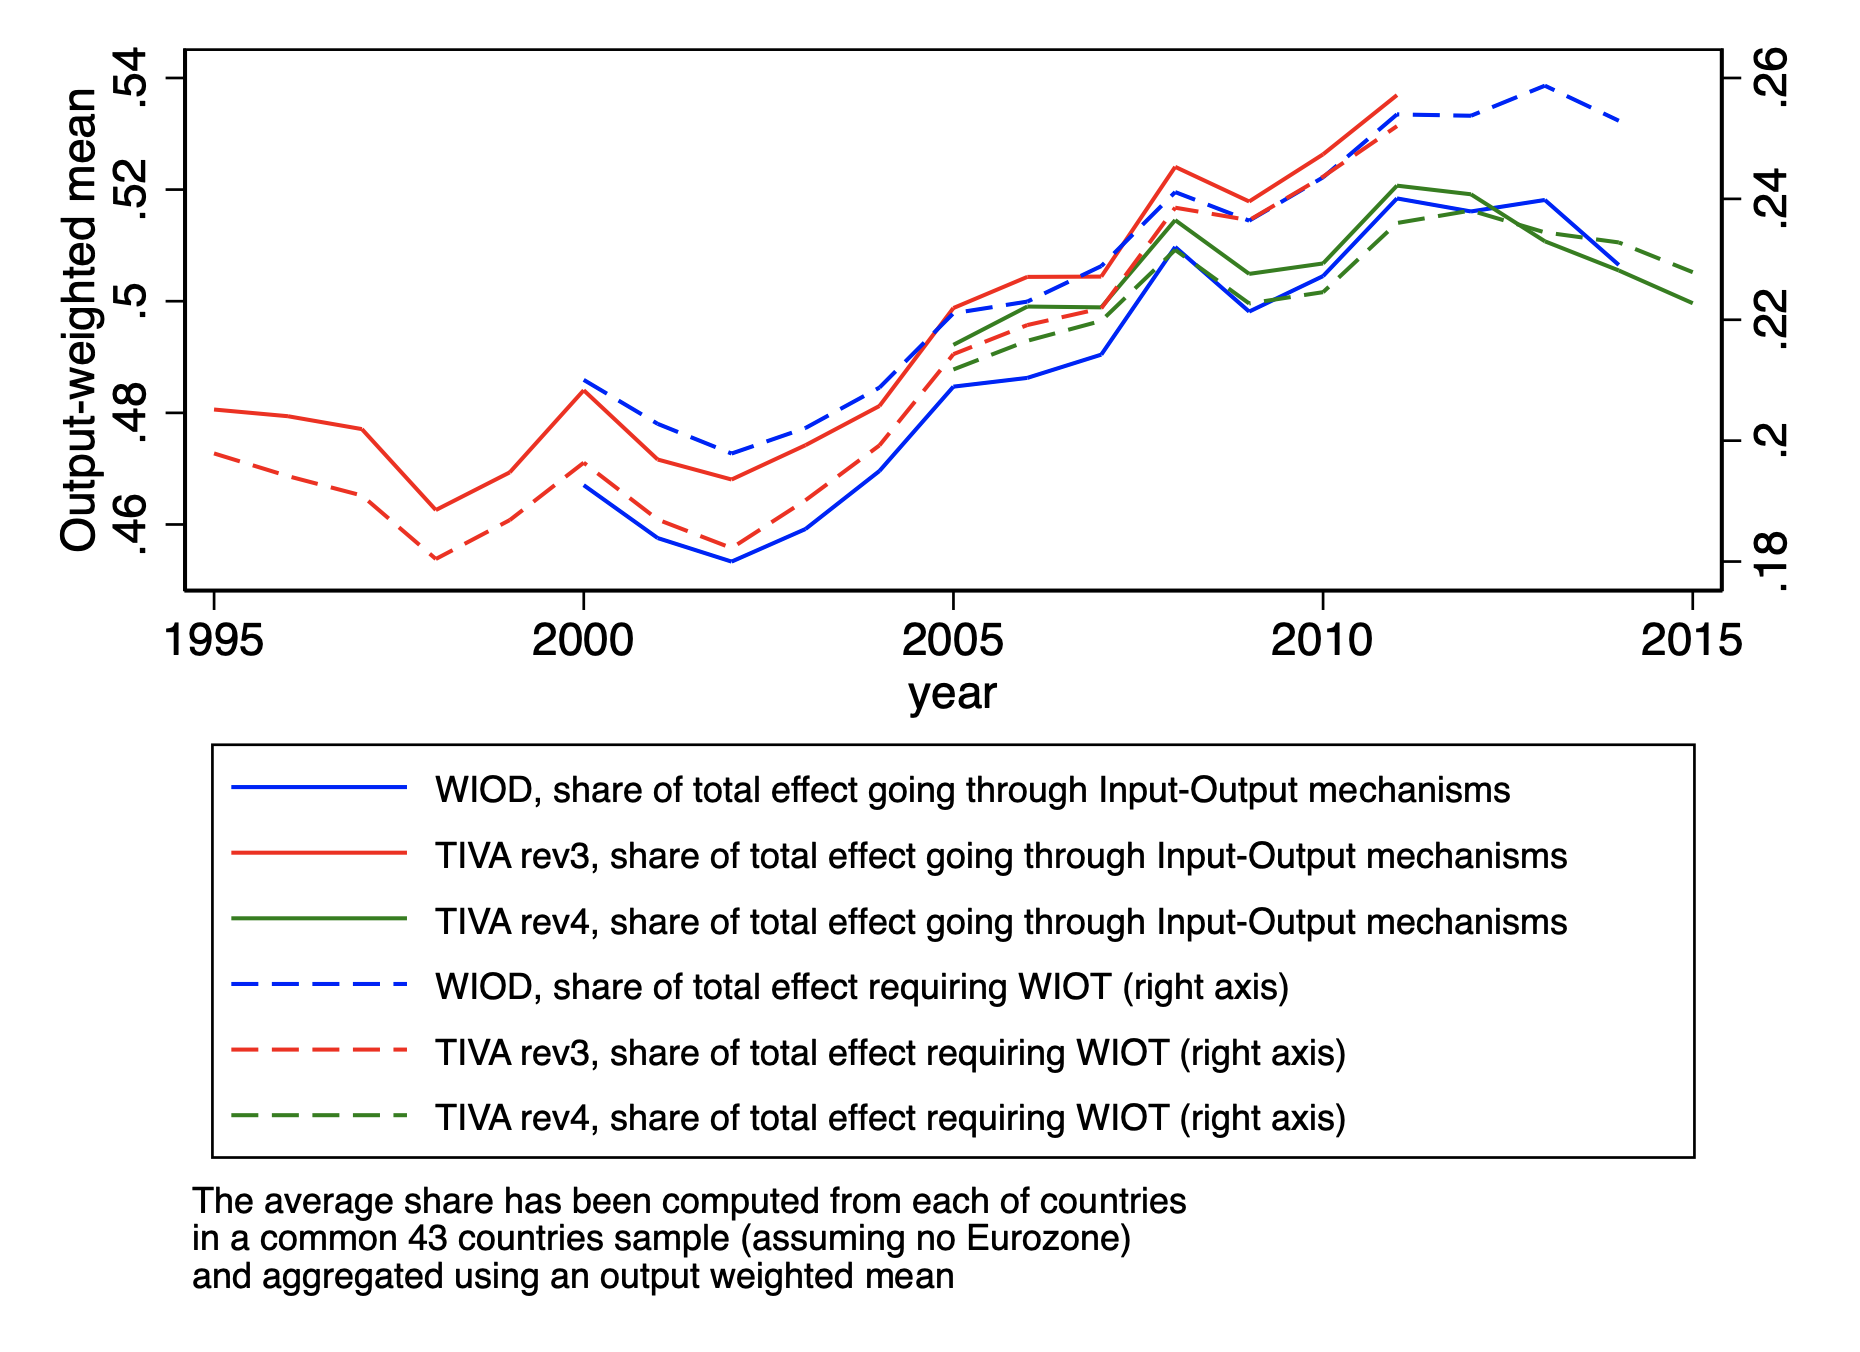
\includegraphics[width=5.0in, height=3.5in]{Share_GDP-weighted.png}\\
		\floatfoot{Sources: WIOD, TIVA rev. 3, TIVA rev. 4 and authors’ calculations} \\
	\end{tabular}
	\label{fig:shareofsthroughtime}
\end{figure}

Overall, the first two channels explain three-quarters of the transmission of an exchange rate appreciation to domestic prices.
By contrast, the last two channels, which reflect the impact of global value chains, play a more limited role, with marked across-countries heterogeneity.
Approximately one-fourth of the HCE deflator elasticity to the exchange rate is attributable to participation in global value chains.\\
Still, $E1.HC$ and $E2.HC$ are relatively important (especially for small countries). Although the model as it stands cannot easily accommodate simultaneous exchange rate changes in different currencies (which would require increasing the number of $\cal{B}$ matrices and $C$ vectors), we expect the effect of simultaneous variations of different currencies to be correctly approximated by an own-currency exchange rate change of the trade-weighted average of the country-specific exchange rate changes.\\


\subsection{Estimating the HCE deflator elasticity using the shares of imported goods and imported inputs in household consumption}

The importance of $E1.HC$ and $E2.HC$ suggests that the HCE deflator elasticity to the exchange rates could be estimated using national accounts data and input-output matrices.
National accounts data provide $E1.HC$ and $E2.HC$, whereas world input-output matrices are needed for computing $E3.HC$ and $E4.HC$. 
We investigate whether $E3.HC$ and $E4.HC$ can be inferred from easier-to-compute elements of $\overline{s}_{i}^{i,HC}$.

%This is suggested by the correlation matrix of  $E1.HC^{i,imp}$, $E2.HC^{i,dom}$, $E3.HC^{i,imp}$ and $E4.HC^i$ (see Table \ref{table:corretable1}). 
%
%\begin{table}[htbp]\centering \caption{Cross-correlation of $\overline{s}_{i}^{i,HC}$'s components (WIOD 2014)\label{table:corretable1}}
\begin{tabular}{l  c  c  c  c }\hline\hline
\multicolumn{1}{c}{Variables} &E1HC&E2HC&E3HC&E4HC\\ \hline
E1HC&1.00\\
E2HC&0.74&1.00\\
E3HC&-0.09&0.11&1.00\\
E4HC&0.36&0.53&0.05&1.00\\
\hline \hline 
 \end{tabular}
\end{table}

% comme on vient de dire que e3 est petit, je sugère de supprimer la phrase ci-dessous
%$E3.HC^{i,imp}$ does not require inverting a matrix, but it is still quite data-intensive to compute. 
We infer $\overline{s}_{i}^{i,HC}$ from $E1.HC$ and $E2.HC$ using equation \ref{eq:infer1}.
Figure \ref{fig:ratiodir_WIOD} depicts the relationship between $\overline{s}_{i}^{i,HC}$ and $E1.HC+E2.HC$. 
The high $R^2$ (0.98) suggests that $E1.HC+E2.HC$ is a good predictor of $\overline{s}_{i}^{i,HC}$. 

 \begin{equation}
\overline{s}_{i}^{i,HC}=\alpha + \beta  \left(E1.HC^{i,imp}+E2.HC^{i,dom}\right) +\varepsilon_i 
\label{eq:infer1}
 \end{equation}
 


\begin{figure}[H]
\centering
\caption{\footnotesize{\textbf{Comparison of $\overline{s}_{i}^{i,HC}$ and $E1.HC^{i,imp}+E2.HC^{i,dom}$ (WIOD, 2014)}}}
\begin{tabular}{c}
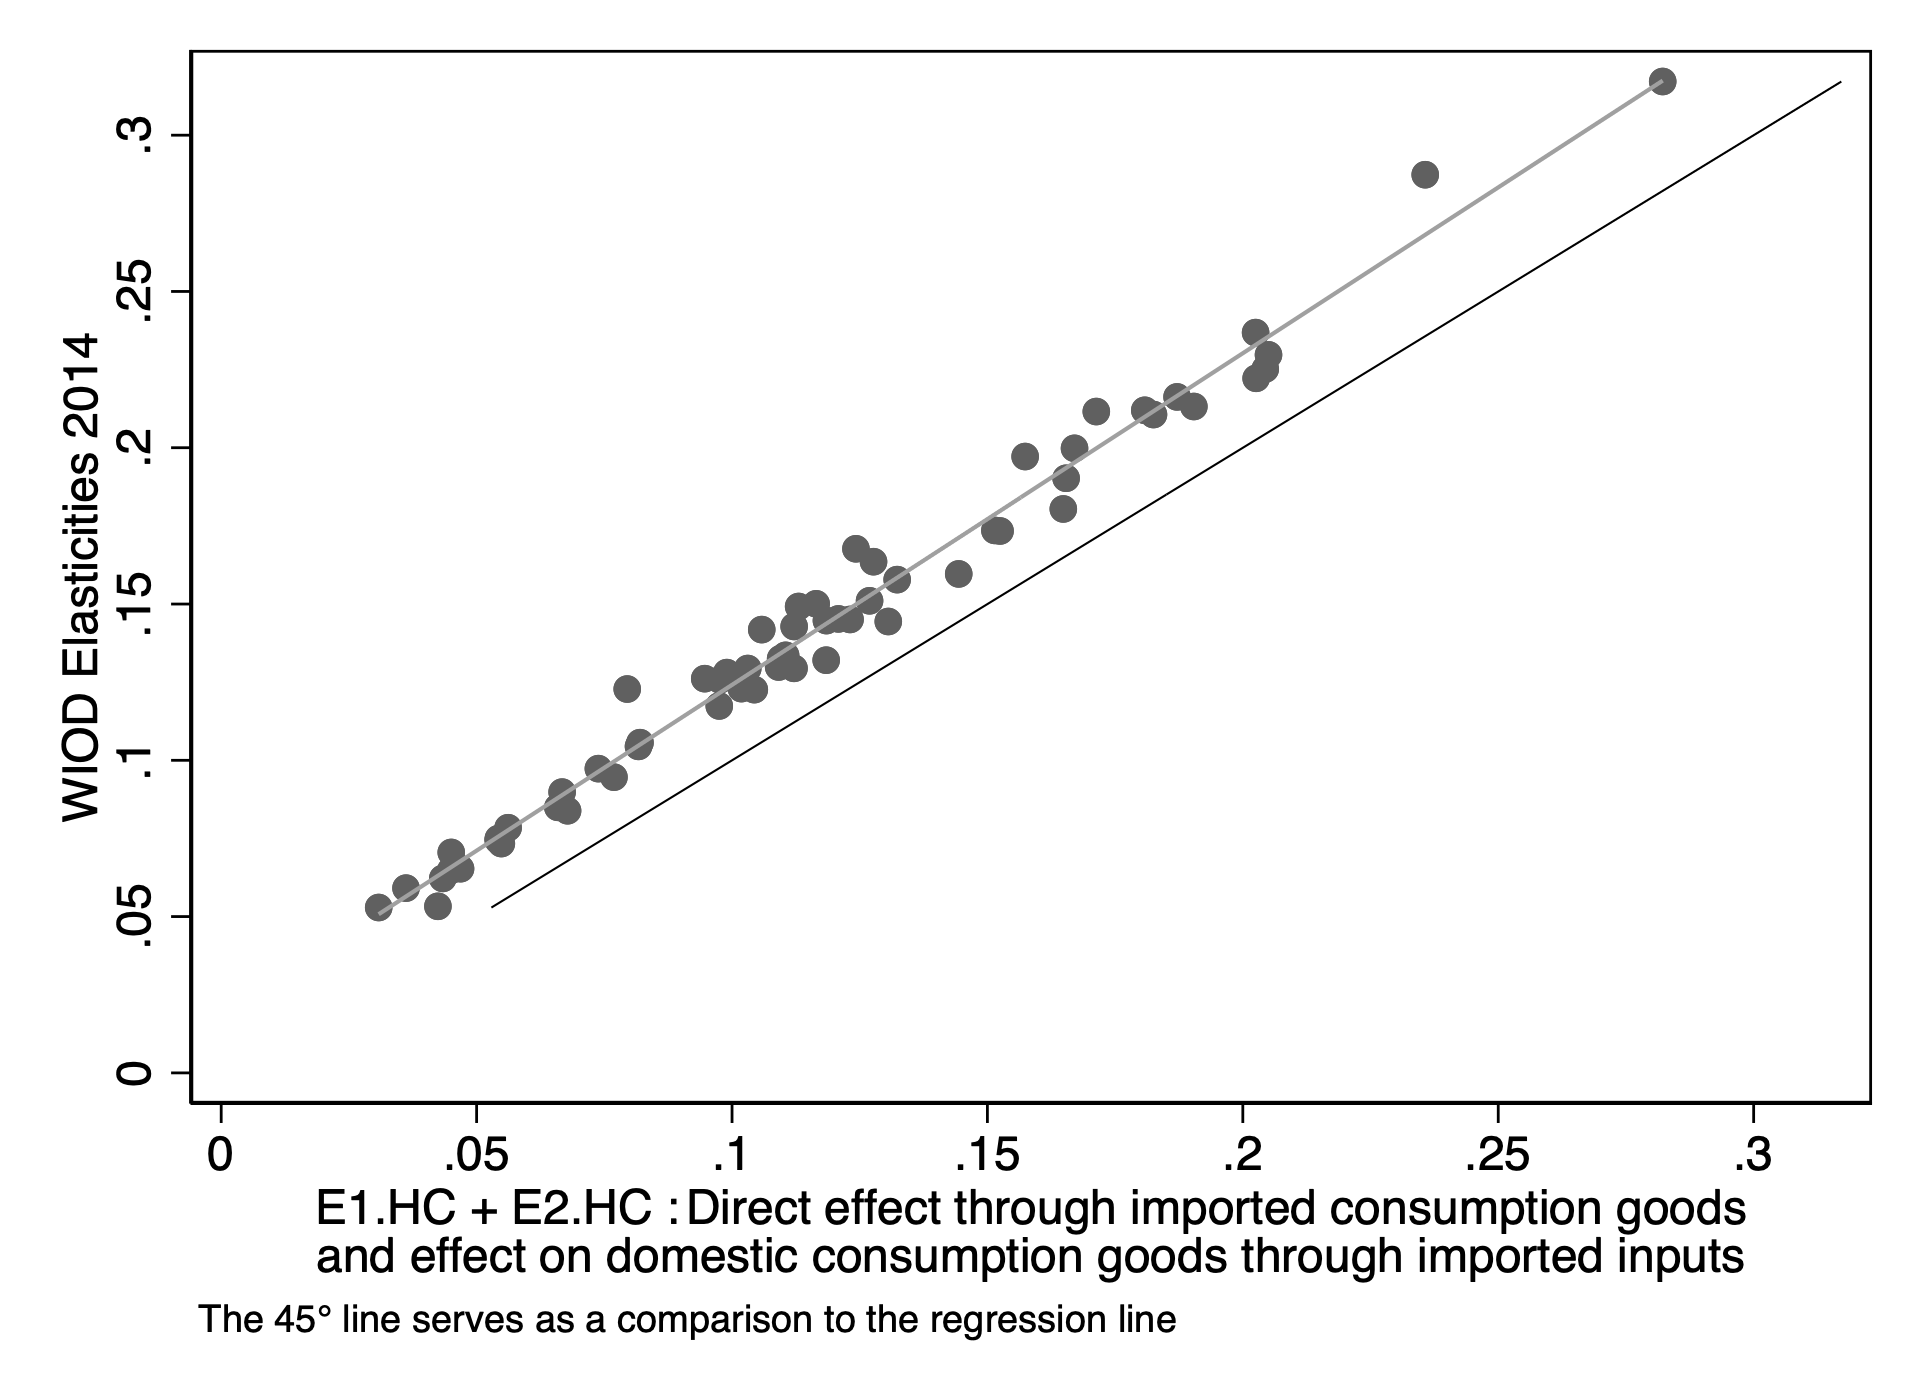
\includegraphics[width=5.0in, height=3.5in]{Comp_s_E1HCE2HC_2014_WIOD_HC.png}\\
\end{tabular}
\floatfoot{Sources: WIOD and authors’ calculations}
\label{fig:ratiodir_WIOD}
\end{figure}

We check whether the relationship is constant over time by estimating yearly cross-sections of equation \ref{eq:infer1}. 
With the exception of 2009, the relationship is broadly stable (see Figures \ref{fig:evolution_coef}).

\begin{figure}[H]
\centering
\caption{\footnotesize{\textbf{Evolution of  $\alpha$ (the constant), $\beta$ (the coefficent of E1.HC+E2.HC) and $R^2$ over time (WIOD)}}}
\begin{tabular}{c}
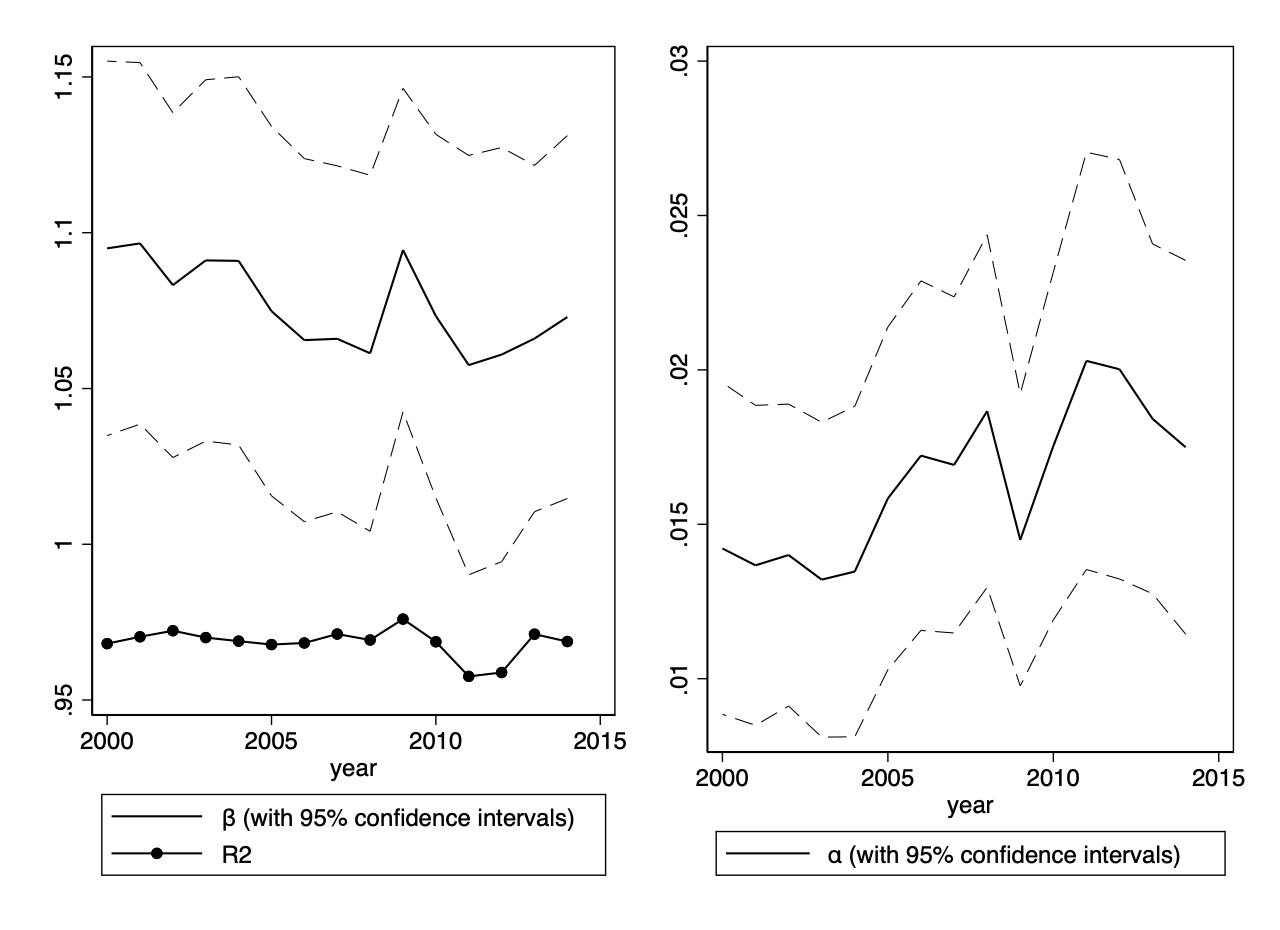
\includegraphics[width=5.0in, height=3.5in]{coef_WIOD_HC.png}\\
\end{tabular}
\label{fig:evolution_coef}
\floatfoot{Sources: WIOD and authors’ calculations}
\end{figure}

We obtain similar results with TiVA (see Online Appendix B). 
% je suggère de retirer cette phrase pour simplifier l'exposé, ou éventuellement d'en faire une note de bas de page
%The functional form might seem a bit counterintuitive (one might expect that the elasticity is affine function of openness as summarized by E1), but the analytical examination of the two-country, one sector case, shows that it is plausible (see Appendix \ref{AnalyticalAppendix}).
Our results suggest that we can approximate the HCE deflator elasticity using the share of imported goods in household consumption and the share of imported inputs in household consumption of domestic goods. $E1.HC+E2.HC$ is a good predictor of the total effects.
Interestingly, they cannot be extrapolated in a multiplicative way, as the other effects ($E3.HC+E4.HC$) add to them rather than amplifying them.
They are of similar size for small open economies and large closed ones.
This likely reflects the fact that a small economy compensates for its small size (and small influence on global value chains) by being more open (and hence more sensitive to changes in global value chains).\footnote{Although this functional form might seem counterintuitive (we expected the elasticity to be an affine function of openness as summarized by $E1.HC$), the analytical examination of the two-country, one-sector case shows that it is plausible (see Online Appendix E).}
%Back to the main point, it turns out that we do not gain much by inversing matrixes. Of course, this realization is only possible because we were able to computes $\overline{s}_{i}^{i,HC}$ in the first place. Still, it suggests that we could extrapolate the elasticities for not-yet-released years, as long as we have the share of imported goods in household consumption and the share of imported inputs in household consumption of domestic goods. 

\subsection{Extrapolating the HCE deflator elasticity using GDP and trade statistics}\label{sec:Extrapolations}
In this section, we show that a precise assessment of the HCE deflator elasticity to the exchange rate can be estimated without resorting to WIOTs. 
The construction of World Input-Output tables is data-demanding and WIOTs are typically released with a lag of several years.
As a result, world input-output matrices are not available for the most recent years.
The latest years covered by WIOD and TiVA rev. 4 are, respectively, 2014 and 2015. 
While the MRIO database covers more recent years, it is fraught with data quality issues for 2018 (see Section \ref{subsec:timeevol} and Online Appendix F).
Using WIOTs also involves cumbersome computations.
Given these difficulties, we look for a simpler way to compute the elasticity of the HCE deflator to the exchange rate.
We estimate the HCE deflator elasticity from 2015 onwards using GDP statistics and trade data on consumption and intermediates.\\
As a starting point, the sum of the share of imported goods in household consumption and the share of imported inputs in household consumption of domestic goods ($E1.HC + E2.HC$) is a good predictor of the impact of exchange rate fluctuations on household consumption prices. 
However, these data ($E1.HC$ and $E2.HC$) are not up-to-date for a large number of countries, as they are not routinely computed by national statistical institutes.
We can rely on a proxy to identify consumption and intermediate goods imports using the CEPII BACI database and the BEC classification \citep{Gaulier2010}\footnote{BACI provides disaggregated data on bilateral trade flows for more than 5000 products and 200 countries. The database is built from data directly reported by each country to the United Nations Statistical Division (Comtrade). Products are defined as items from the Harmonized System nomenclature, at the 6-digit level.}
Household consumption and intermediate products are more difficult to collect systematically for many countries and many years. In Online Appendix C, we use data from the World Bank and Eurostat, which are only available for a limited number of countries. Hence, the study reported in Online Appendix C only includes a limited number of observations.

Here, to expand our panel, we use an even simpler proxy for $E1.HC+E2.HC$, using only trade data from BACI and GDP data from the World Bank (see equation \ref{eq:infer2}).
These data are available until 2019. 
 \begin{equation}
\begin{array}{llll}
\overline{s}_{i,t}^{i,t,HC}= \alpha & +  \beta_1  \frac{\textnormal{imported consumption goods}_{i,t}}{\textnormal{GDP}_{i,t}} \\ & + \beta_2 \frac{\textnormal{imported intermediate goods}_{i,t}}{\textnormal{GDP}_{i,t}} \\
& +  \beta_3  \frac{\textnormal{Total sample imported consumption goods}_{t}}{\textnormal{Total sample GDP}_{t}} \\
& + \beta_4 \frac{\textnormal{Total sample imported intermediate goods}_{t}}{\textnormal{Total sample GDP}_{t}} \\
& +fe_{i}+\varepsilon_{i,t}
\end{array}
\label{eq:infer2}
\end{equation}

We perform an out-of-sample prediction for WIOD, 2014, using data for years 2000 to 2008.
The results are satisfactory, although the mean and median errors are larger than in Online Appendix C (see Figure \ref{fig:panel_pred2}). 
Our findings are robust to using other databases (results obtained with TiVA revisions 3 and 4 are available upon request).


\begin{figure}[!h]
	\centering
	\caption{\footnotesize{\textbf{Comparing the HCE deflator elasticity in 2014 (WIOD) and the prediction from a panel regression on the 2000-2008 period with fixed effects using only World Bank and Comtrade data. }}}
	\begin{tabular}{c}
		\includegraphics[width=5.0in, height=3.5in]{"resultats_reg1_doigt_mouille_WIOD_pred_6y_trend_no".png}\\
	\end{tabular}
	\label{fig:panel_pred2}
	\floatfoot{Sources: WIOD, World Bank, BACI and authors’ calculations}
\end{figure}

Using these equations, we can predict the HCE deflator elasticity from 2015 onwards.
Figure \ref{fig:panel_pred3} shows that the in-sample predictions are robust, giving confidence in the quality of the out-of-sample predictions.
We also compare our predictions with the elaticity estimated using MRIO, which provides WIOTs up to 2019. 
Our predictions are in line with results from MRIO up to 2017. For the most recent years, there seem to be data issues in MRIO (see Online Appendix F), which the comparison helps to identify.
We thus provide a simple accounting tool to estimate the percentage change in prices in response to exchange rate variations for the most recent years.


\begin{figure}[H]
	\centering
	\caption{\footnotesize{\textbf{Comparing the output-weighted HCE deflator elasticity to predictions based on World Bank and BACI data.}}}
	\begin{tabular}{c}
		\includegraphics[width=5.0in, height=3.5in]{"predictions_reg1_doigt_mouille_trend_no".png}\\
	\end{tabular}
	\label{fig:panel_pred3}
		\floatfoot{Sources: WIOD, TIVA, MRIO, World Bank, BACI and authors’ calculations}
\end{figure}





%
%\clearpage
%
%
%\clearpage
%+++++++++++++++++++++++++++++++++++++++++++++++++++++++++
%\subsection{The intensity of import in domestic consumption}
%\label{subsec:intensity}
%
%\begin{figure}[!h]
%\centering
%\caption{\footnotesize{\textbf{The share of imported intermediate and consumer goods and services in private consumption }}}
%\begin{tabular}{c}
%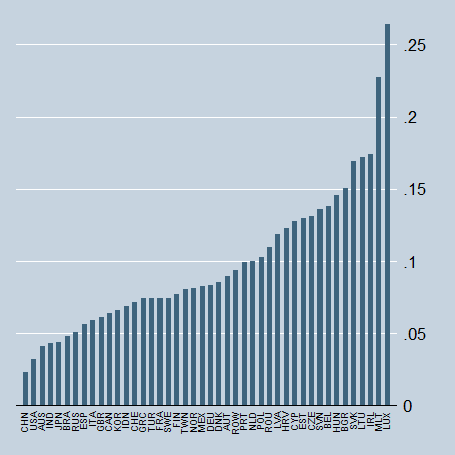
\includegraphics[width=5.0in, height=3.5in]{Graph_ratioimp_wiod_2014}\\
%\floatfoot{Source: WIOD, 2014}.
%\end{tabular}
%\label{fig:ratioimp}
%\end{figure}
%
%Differences in the import intensity across sectors and countries are crucial to our analysis on global nominal spillovers.
%In this section, we present some stylised facts about the import intensity in domestic consumption.
%Using data from the WIOD, we define the import intensity of private consumption as the share of  imported intermediate and final goods and services in total consumption. \\
%Figure \ref{fig:ratioimp} depicts the import intensity  of  household consumption in 2014.
%Not surprisingly, small countries, such as Malta, Luxembourg and Ireland, have the highest import intensity (above 15$\%$), while larger countries, such as Japan, the U.S. and Australia, display a much lower ratio of import intensity.\\
%How has the import intensity of private consumption changed over time? 
%In the Euro area, Figure \ref{fig:ratioimptemp_ze} shows that the import intensity of consumption increased in most member states over the last decade. Following the adoption of the euro, the intensity of import increased between 2000 and 2007 in all countries except the southern economies (Spain, Portugal and Greece). In the years following the Great Recession, the import intensity of consumption kept expanding in the two largest economies of the area (Germany, France), but receded in the countries stricken by the sovereign-debt crisis (Spain, Italy, Portugal and Greece).\\
%Outside of the euro area, Figure \ref{fig:ratioimptemp} shows that the import intensity of consumption has broadly expanded since 2000. 
%In all countries, except China, Croatia, Indonesia and Russia, the import intensity was higher in 2014 than it was in 2000.
%In China, it declined somewhat following the 2008-2009 crisis, reflecting global value chains shortening. In Russia, the intensity of import has been decreasing over the last two decades. 
%\begin{figure}[!h]
%\centering
%\caption{\footnotesize{\textbf{Evolution of the intensity of import in household consumption in the euro area}}}
%\begin{tabular}{c}
%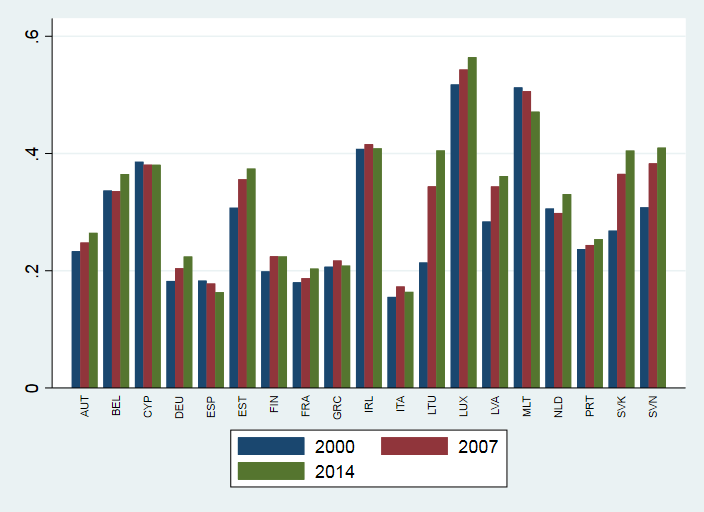
\includegraphics[width=5.0in, height=3.5in]{Graph_ratioimp_WIOD_2000_2014_ze}\\
%\floatfoot{Source: WIOD}.
%\end{tabular}
%\label{fig:ratioimptemp_ze}
%\end{figure}
%
%
%\begin{figure}[!h]
%\centering
%\caption{\footnotesize{\textbf{Evolution of the intensity of import in household consumption}}}
%\begin{tabular}{c}
%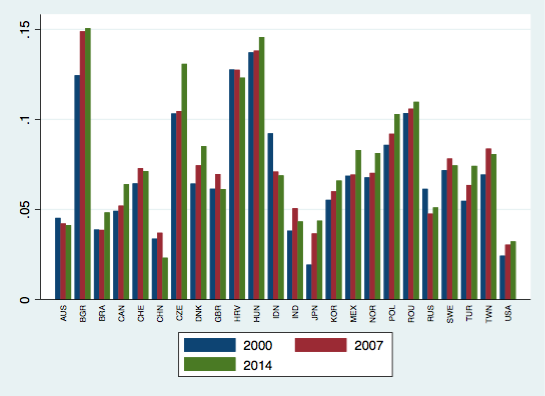
\includegraphics[width=5.0in, height=3.5in]{Graph_ratioimp_WIOD_2000_2014}\\
%\floatfoot{Source: WIOD}.
%\end{tabular}
%\label{fig:ratioimptemp}
%\end{figure}
%
%
%\subsection{The reaction of domestic consumer prices to changes in import prices}
%In this section, we evaluate how domestic consumer prices react to changes in prices of imported intermediate and final goods, the latters being caused by exchange rate fluctuations. 
%We are interested in (\textit{i}) the direct effect of global inflationary shocks, defined as the share of imported final and intermediate goods in domestic consumption (i.e. the import intensity in domestic consumption defined in Section \ref{subsec:intensity}) and (\textit{ii}) the total effect. The latter depends both on the direct effect and on the additional transmission of lower domestic input prices to other sectors of the domestic economy as well as to other countries which occurs during subsequent production cycles. 
%\paragraph{How much of domestic consumer prices' reactions to changes in import prices is explained by the direct effect?}
%
%Figure \ref{fig:ratiodir} depicts how much of the total impact of a change in import prices is explained by the import intensity of household consumption. In other words, Figure \ref{fig:ratiodir} represents the ratio of the direct effect to the total effect.
%In all countries, the direct effect accounts for more than 60$\%$ of the total impact in 2014. 
%%In five economies (India, Indonesia, Luxembourg, Mexico and Turkey), the direct effect explains more than 80$\%$ of the reaction of domestic consumer prices to changes in import prices, which suggests that these countries do not provide much intermediate goods to their partners. 
%For the whole cross-section, the coefficient of correlation between the total and the direct effect is close to unity in 2014.
%
%\begin{figure}[!h]
%\centering
%\caption{\footnotesize{\textbf{Ratio of direct to total effect of domestic consumer prices reactions to changes in import prices}}}
%\begin{tabular}{c}
%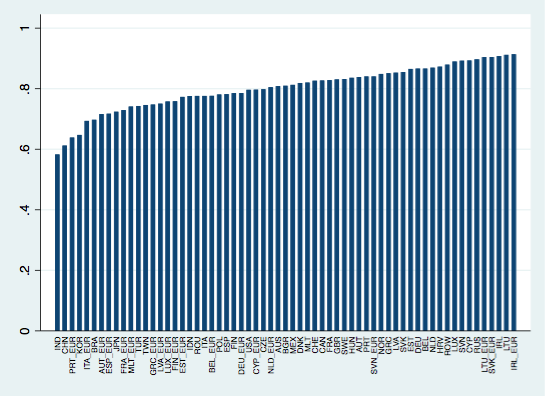
\includegraphics[width=5.0in, height=3.5in]{Graph_ratiodir_WIOD_2014}\\
%\floatfoot{Source: WIOD, 2014}.
%\end{tabular}
%\label{fig:ratiodir}
%\end{figure}
%
%
%\section{The impact of exchange rates fluctuations on the main components of consumer prices}
%\label{sec:prixconsosecteur}
%\paragraph{Differences in the intensity of import use across sectors} 
%In this section, we investigate the import intensity of consumption at the sectoral level. We run the following sectoral regressions (Equation \ref{eq:eq8}) for each sector $j$. 
%
% \begin{eqnarray}
%{S^{HC}_j}=\beta_j  I + c_j +\varepsilon
%\label{eq:eq8}
% \end{eqnarray}
% with ${S^{HC}}$ the impact of the devaluation shock on consumer prices, for each country $i$, and $I$ the vector of country-specific and sector-specific import intensity of consumption.
% 
%
%\begin{figure}[!h]
%\centering
%\caption{\footnotesize{\textbf{Consumer prices elasticity to an exchange rate shock: a sectoral analysis}}}
%\begin{tabular}{c}
%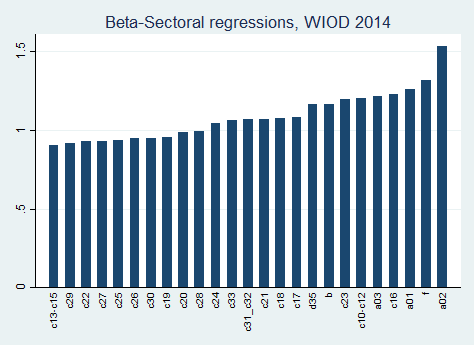
\includegraphics[width=5.0in, height=3.5in]{Graph_beta_2014_Wiod_reg_sec}\\
%\floatfoot{Source: WIOD, 2014. \\
%}
%\end{tabular}
%\label{fig:betasecteur}
%\end{figure}
%
%\begin{figure}[!h]
%\centering
%\caption{\footnotesize{\textbf{Sectoral analysis: R2}}}
%\begin{tabular}{c}
%\includegraphics[width=5.0in, height=3.5in]{Graph_r2_2014_Wiod_reg_sec}\\
%\floatfoot{Source: WIOD, 2014. \\
%}
%\end{tabular}
%\label{fig:betar2}
%\end{figure}

\section{Conclusion}
\label{sec:ccl}
% Avril 2021
This paper studies the elasticity of the household consumption expenditure (HCE) deflator to the exchange rate.
Our contribution to the literature is fourfold. \\
First, we analyse the composition and determinants of the HCE deflator elasticity using world input-output tables covering twenty-four years of data, from 1995 to 2019. 
We use several datasets to ensure the robustness of our results.
In line with the existing literature, we find a rather modest output-weighted elasticity of the HCE deflator to the exchange rate of around 0.1 at the world level.
The output-weighted elasticity has remained broadly stable over the past two decades.
Aggregate figures mask substantial cross-country heterogeneity, reflecting different degrees of openness to trade and differences in foreign product content in domestic consumption. 
The elasticity is larger for small open economies with higher import content of consumption. \\
Second, we examine which parts of the consumption basket contribute most to the elasticity of the HCE deflator to the exchange rate. 
Non-energy industrial goods explain the bulk of the total HCE deflator elasticity. 
Services also play a significant role, as they represent a substantial share of total consumption. \\
Third, we analyse the determinants of the HCE deflator elasticity and the role of global value chains in the transmission of an exchange rate appreciation to domestic prices.
There is a marked cross-countries heterogeneity.
On the whole, direct effects through imported consumption and intermediates entering domestic production explain three-quarters of the transmission of an exchange rate appreciation to domestic prices.
By contrast, global value chains participation plays a limited role. \\
Fourth, we show that a precise assessment of the HCE deflator elasticity to the exchange rate can be extrapolated for recent years, for which good-quality WIOTs are missing.
We estimate the HCE deflator elasticity using GDP statistics and trade data on consumption and intermediates and obtain reliable out-of-sample predictions.

% conclusion precedente
%In this paper, we investigate the role of GVCs for inflation dynamics within a unified framework of input-output databases (WIOT and TIVA) from 1995 to 2018.  
%Our main results are threefold.
%First, we confirm the importance of Global Value Chains in explaining inflation dynamics.
%%GVC cannot be neglected in the debate about he determinants of inflation.
%The Household consumption expenditure deflator elasticity to a shock on the domestic currency ranges from 0.05 to 0.35, depending mainly on the openness of countries.
%Within the euro area, the range of elasticities is large, adding to the challenges faced by the European Central Bank in stabilising prices throughout the monetary union.
%Input-output mechanisms explain a large share of the elasticity, especially for large countries.
%Our results are robust to using different databases (WIOD, TiVA 2016 and TiVA 2018).
%Second, we show that the direct impact (through imported final goods) and domestic Input-Output linkages (i.e. domestic final goods produced using foreign inputs) account for most of the propagation of an exchange rate shock to domestic prices.
%First-round effects explain three-quarters of the propagation of exchange rate shocks to domestic prices.
%By contrast, we find a limited role for the second-round effects, i.e. the additional transmission of lower domestic input prices to other sectors of the domestic economy and other countries occurring during subsequent production cycles.
%We analyse the contribution of different sectors to the HCE deflator elasticity to an exchange rate shocks. Domestic core inflation (defined as inflation excluding food and energy) accounts for a significant share of the total elasticity, mainly reflecting the weight of domestic services and non-energy industrial goods in total consumption.
%Third, we provide a tool to estimate the elasticity of the HCE deflator to the exchange rate without resorting to WIOTs. 
%The construction of World Input-Output tables is data-demanding and WIOTs are not available for the most recent years. 
%To address this gap, we use more up-to-date GDP and trade data to approximate the HCE deflator elasticity from 2016 onwards.
%%Overall, our results confirm and quantify the usefulness of the Input-Output approach for understanding inflation dynamics, which is key as for monetary policy. 

%%GD20200621Peut-être faudrait-il faire le boulot de la figure 2 pour la période 2016-2019 ???


\newpage
%\bibliographystyle{agsm}
%\bibliographystyle{elsarticle-harv}
%\bibliographystyle{plainnat}
\bibliographystyle{apalike}
\bibliography{PapiertransmissiondeschocsenVA.bib}

\end{document}
